		\chapter{Обсуждение результатов.}
Исследованные нами поселения были достаточно разнообразны по географии и абиотическим характеристикам.
В Белом море изучаемые поселения были расположены в основном в вершине Кандалакшского залива, кроме того, мы располагаем данными о поселениях маком в губе Чупа. 
В Баренцевом море обследованы поселения вдоль значительной части Мурманского побережья.
Наиболее полно были обследованы губы Восточного Мурмана.

В исследовании представлены поселения, расположенные как на материковой литорали (бухта Лисья, пролив Подпахта, Лувеньга), так и на островах (два участка на о.~Кереть, два участка на о.~Ряшков, о.~Ломнишный, о.~Горелый Лувеньгских шхер). 
Два участка (эстуарий р.~Лувеньги, Сухая салма) расположены в области влияния эстуариев рек (Лувеньга и Кереть, соответственно)  и характеризуются пониженной соленостью по сравнению с остальными.
Разнообразна и степень прибойности: от прибойной литорали в б.~Клющиха до затишных губ (участки в Сухой салме, в Южной губе о.~Ряшкова, на о.~Горелом).
Таким образом, участки биотопически разнородны и относительно полно характеризуют разнообразие илисто-песчаных литоралей в Кандалакшском заливе.

В Баренцевом море исследованные нами поселения расположены в основном в относительно крупных материковых губах.
Согласно представлениям Е.Ф.~Гурьяновой и П.В.~Ушакова (\cite{Guryanova_Ushakov_1929}) на Восточном Мурмане преобладают открытые неглубокие губы с крайне обедненной фауной, и лишь в отдельных более закрытых губах наблюдается развитие богатых сообществ на мягких грунтах.
Все исследованные нами губы относились к достаточно закрытым акваториям, то есть в местах, где можно ожидать максимального развития поселений маком.

Cоленостная толерантность взрослых особей {\it M.~balthica} достаточно высока (\cite{Naumov_2006}), однако соленость может играть роль на начальных стадиях развития.
В целом, исследованный район в Баренцевом море характеризуется соленостью близкой к океанической.
Характерно, что все поселения на Западном и Восточном Мурмане расположены в губах, в которые впадают небольшие реки или ручьи, то есть находятся в распресненных условиях.
Соленость в Кольском заливе ниже океанической за счет впадения в кут залива крупных рек Колы и Туломы, и таким образом участки, расположенные вне губ с локальным стоком, тоже находились в распресненных условиях.
Тем не менее, невозможно утверждать, что распределение маком на Мурмане находится под влиянием солености, так как невозможно изолировать несколько важных абиотических фактора: соленость, характер грунта и степень прибойности/закрытости акватории, поскольку для Мурманского побережья характерно наличие берегового стока в закрытых губах (\cite{Guryanova_Ushakov_1929, Guryanova_et_al_1930}).
Белое море в целом характеризуется пониженной соленостью и ее среднегодовое значение не превышает 25\permil.
В данной акватории нельзя говорить о приуроченности поселений маком в локальному береговому стоку, и среди исследованных участков были как участки, находящиеся под влиянием рек и ручьев, так и вне зоны влияния оных.

\textit{M.~balthica}~--- обитатель мягких грунтов.
По данным А.~Д.~Наумова, в Белом море $35$\% находок данного вида относятся к биотопам с илистыми грунтами и $46$\%~--- с песчаными. 
Исследованные нами участки представляли собой песчаные отмели с различной примесью ила, то есть относились к типичным местообитаниям маком.
Интересно, что в Белом море максимальные биомассы \textit{M.~balthica} отмечены на мелко-гравийном грунте (\cite{Naumov_2006}), что хорошо прослеживается на наших данных: биомасса на литорали в Западной Ряшковой салме выше, чем на других участках.

Моллюски {\it M.~balthica}~--- амфибореальный вид. 
По Американскому побережью Атлантики вид распространен на север до Лабрадора.
В Европейской части ареала {\it M.~balthica} заходит в арктические моря, и встречается в Норвежском, Баренцевом, Белом и Карском морях.
Наиболее северной точкой считается Шпицберген (\cite{Zacepin_Filatova_1968}).

В Баренцевом море макомы вместе с другими представителями бореальной и бореально-арктической фауны заселяют пляжи осушной зоны и верхней сублиторали. 
По данным Е.~Ф.~Гурьяновой, И.~Г.~Закса и П.~В.~Ушакова (\cite{Guryanova_et_al_1928, Guryanova_Ushakov_1929, Guryanova_et_al_1930}, макома повсеместно встречается на мягких грунтах в бухтах Кольского залива и Мурманского побережья. 
Все отмеченные нами виды характерны для литорали Кольского залива и Восточного Мурмана (\cite{Derugin_1915, Guryanova_Ushakov_1929}).

В Белом море \textit{M.~balthica} входит в литоральный комплекс двустворчатых моллюсков и отмечена во всех заливах (\cite{Naumov_2006}).
По данным различных исследователей (\cite{Babkov_Golikov_1984, Naumov_Fedyakov_1993}) для среднего и нижнего горизонта литорали с мягкими грунтами характерно формирование сообществ с доминированием \textit{M.~balthica}. 
Все встреченные нами виды являются характерным окружением для \textit{M.~balthica} (например, \cite{Chertoprud_et_al_2004, Naumov_2006, Gerasimova_et_al_2010, Derevenschikov_Kravets_2010, Stolyarov_2010}).

\bigskip
Таким образом, абиотические и биотические характеристики в изученных местообитаниях позволяет говорить, что  мы имели дело с типичными для исследованных акваторий биосистемами. 


\afterpage{\clearpage}

\section{Структура поселений \textit{Macoma~balthica} }
		\subsection{Обилие {\it Macoma balthica} в европейской части ареала}
Полученные для Белого и Баренцева данные хорошо согласуются с литературными данными об этих регионах.
Так, по нашим данным, на литорали Кольского залива численность {\it M.~balthica} составляла около $1000$~экз./м$^2$, что хорошо соотносится с результатами, полученными ранее для других областей данной акватории. 
Л.~Басова, обладая данными по большему количеству участков в Кольском заливе, приводит средние показатели плотности поселения маком $802 \pm 273$~экз./м$^2$ при максимальной численности $2900$~экз./м$^2$ (\cite{Basova_2004}).
На Восточном Мурмане численность {\it M.~balthica} в основном не превышала $100$~экз./м$^2$, лишь на одном участке достигая $500$~экз./м$^2$. 
И.~Я.~Агарова с соавторами (\cite{Agarova_et_al_1976}) даёт оценку численности {\it M.~balthica} крупнее $5$~мм для разных сообществ Дальнего пляжа губы Дальне-Зеленецкой в 1973 году от $12$ до $42$~экз./м$^2$ (рис.~\ref{ris:dynamic_Zelency_Agarova}). 
	\begin{figure}[p]
%		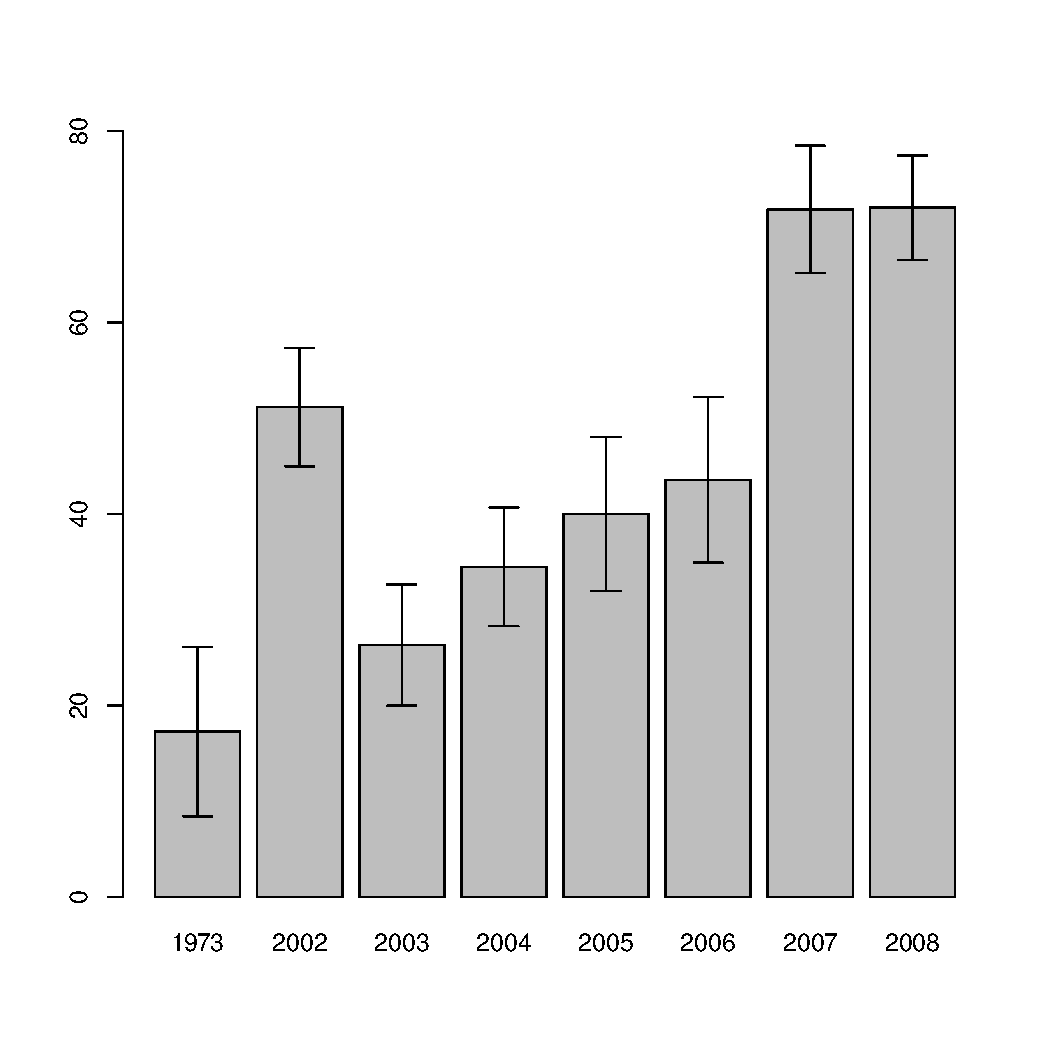
\includegraphics{../Barenc_Sea/Dalnezeleneckaya/N_dynamic_with_Agarova.pdf}
		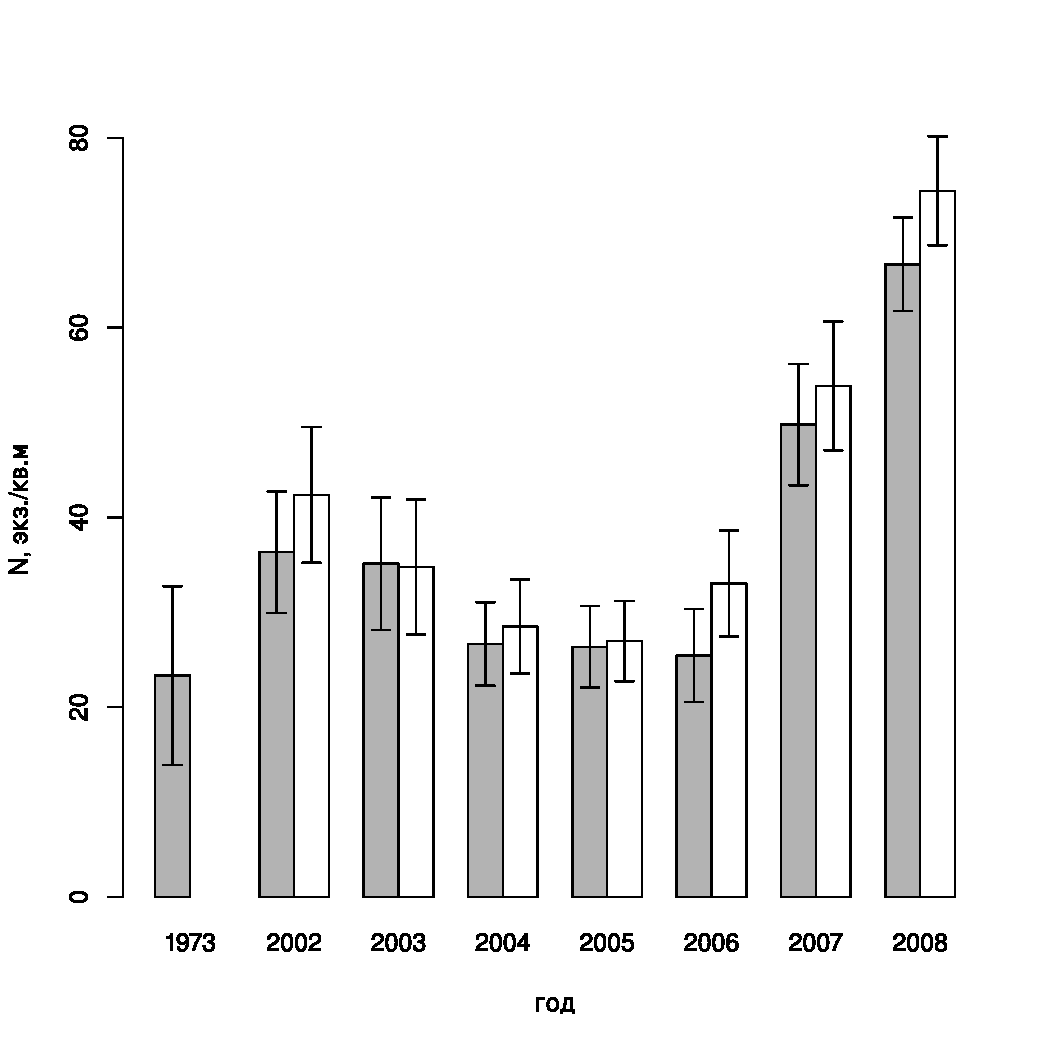
\includegraphics{../after_Deryuginskie/Macoma_N_dynamic_all1.pdf}
	\caption{Динамика плотности поселений {\it Macoma balthica} на литорали Дальнего пляжа г.~Дальне-Зеленецкой (Баренцево море)}
{\footnotesize Примечание: по оси $X$~--- годы наблюдений, по оси $Y$~--- средняя плотность поселения,~экз./м$^2$. \\
Светлые столбцы~--- общая численность, темные столбцы~--- численность моллюсков крупнее $5$~мм. Данные $1973$ года взяты из статьи \cite{Agarova_et_al_1976}}
	\label{ris:dynamic_Zelency_Agarova}
	\end{figure}
Плотность поселения {\it Macoma balthica} на Дальнем пляже в $1973$ году была сравнима с таковой в $2002-2006$ годах (табл.~\ref{tab:DZ_N_1973_sravnenie}).
	\begin{table}[p]
	\caption{Сравнение численности {\it Macoma balthica} на Дальнем пляже губы Дальне-Зеленецкой в $1973$ году и $2002-2008$.}
	\label{tab:DZ_N_1973_sravnenie}
	\begin{tabularx}{\textwidth}{|*{4}{X|}} \hline
	годы сравнения & $W$ & $p-value$ & достоверность различий \\ 
	\hline
	$1973 - 2002$ & $31,5$ & $0,08$ & *\\
	\hline
	$1973 - 2003$ & $80,5$ & $0,86$ & \\
	\hline
	$1973 - 2004:2006$ &  $214$ & $0,44$ & \\
	\hline
	$1973 - 2007:2008$ & $22$ & $0,0048$ & ** \\
	\hline
	\end{tabularx}
	{\footnotesize Примечание: $W$ - значение критерия Вилкоксона, достоверность различий ***~--- $p<0,001$; **~--- $p<0,05$; *~--- $p<0,1$.}
	\end{table}


Для Белого моря максимальные численности по нашим данным сравнимы с приводимыми в работе А.Д.~Наумова (\cite{Naumov_2006}) максимальными значениями для Белого моря ($4581$~экз./м$^2$ в Оленьей салме в куту Кандалакшского залива). 
Размах варьирования численности маком по данным других мониторинговых программ в Кандалакшском заливе Белого моря аналогичен нашим наблюдениям~--- от нескольких десятков особей до $1-3$ тысяч особей на квадратный метр (\cite{Semenova_1974, Maximovich_et_al_1991, Varfolomeeva_Naumov_2013}). 


%Согласно классическим представлениям {\it M.~balthica} описывается как амфибореальный вид. 
%В Атлантическом океане данный вид встречаются по всему европейскому побережью до Франции на юге. 
%По американскому~--- от штата Джорджия на юге до моря Баффина и западного побережья Гренландии на севере. 
%В Тихом океане {\it M.~balthica} встречается до залива Посьет в Японском море по азиатскому берегу, и до Сан-Диего~--- по американскому. 
%Также данный вид заходит в моря Северного Ледовитого океана:  Норвежское, Баренцево, Белое, Карское, Чукотское и Бофорта. 
%В западном секторе Арктики, самые восточные находки вида~--- из Байдарацкой губы Карского моря, а самые северные~--- со Шпицбергена (\cite{Semenova_1974, Kafanov_1985, Maximovich_1985, Meehan_1985, Naumov_2006, Meehan_et_al_1989, Hummel_et_al_1997_stress}).

%Современные молекулярные исследования показывают неоднородность вида {\it M.~balthica} sensu lato в пределах ареала, причем можно говорить о нескольких уровнях гетерогенности. 
%Рассматривая самый верхний уровень внутривидовой генетической структуры, в настоящее время предлагают выделять атлантический ({\it M.~balthica rubra} и тихоокеанский {\it M.~balthica balthica} подвиды.
%Однако  в морях, связанных с  Атлантикой, существуют очаги распространения тихоокеанской формы. 
%Так, в Балтийском, Белом и Баренцевом морях обитает тихоокеанская форма {\it M.~balthica balthica}. В Баренцевом море она распространена на восток до Варангер-фьорда (\cite{Vainola_2003}). 

Для сравнения наших данных по Белому и Баренцеву морям с данными по обилию маком в других частях европейской части ареала была собрана опубликованная информация о среднем обилии особей {\it M.~balthica} в различных акваториях (прил.~\ref{app:NB_areal}). 
Из анализа исключали данные об обилии сеголетков, и учитывали только информацию об обилии особей старше $1$~года.
Полученные данные визуализировали на карте (рис.~\ref{ris:N_macrodistribution}).
	\begin{figure}[p]
    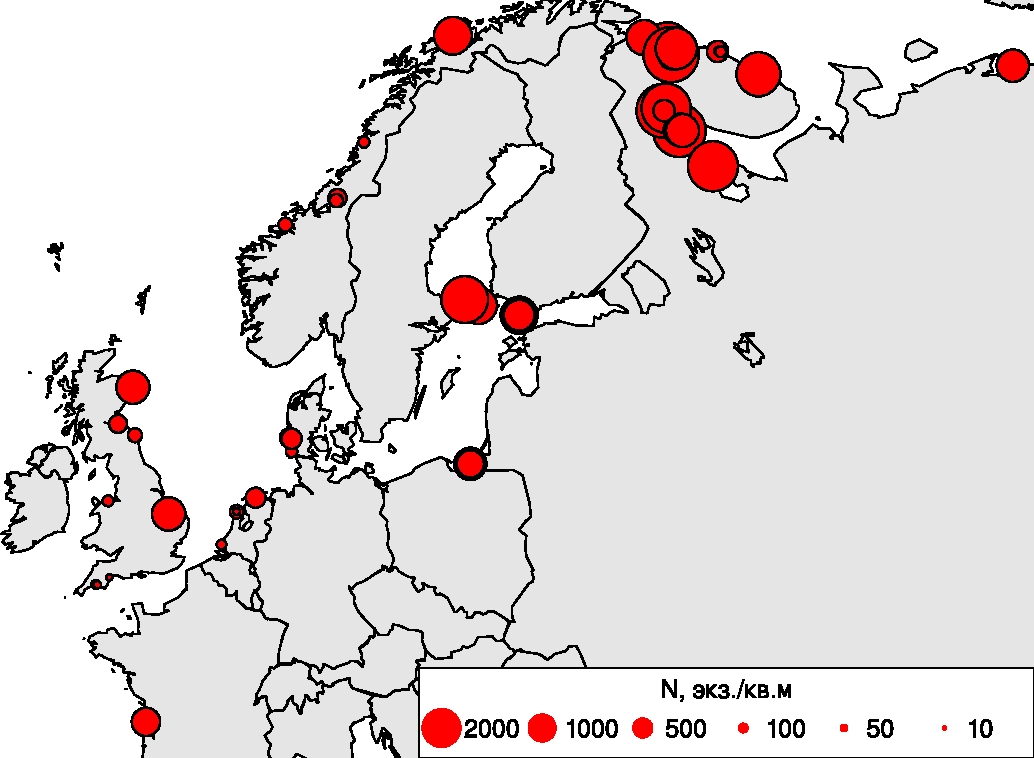
\includegraphics[width=\textwidth]{../macrodistribution/Nmean_ru1.pdf}
    \caption{Численность {\it Macoma balthica} в европейской части ареала}

{\footnotesize Примечание: Площадь кругов пропорциональна средней численности (N) моллюсков,~экз./м$^2$\\
Источники данных см. в прил.~\ref{app:NB_areal}.}
    \label{ris:N_macrodistribution}
	\end{figure}
Численность {\it M.~balthica} на Западном Мурмане и в Кольском заливе была сравнима с численностями моллюсков в Белом море, Балтийском море и северной части Норвежского моря (\cite{Semenova_1974, Aschan_1988, Maximovich_et_al_1991, Bonsdorff_et_al_1995, Bostrom_Bonsdorff_2000, Oug_2001, Laine_et_al_2003, Khaitov_et_al_2007, Varfolomeeva_Naumov_2013}).
Численности маком, сходные по величине с отмеченными на Восточном Мурмане, характерны для Норвежского и Северного морей (включая Ваттово море) (\cite{Brady_1943, Sneli_1968, Stromgren_et_al_1973, Beukema_1976, Jensen_Jensen_1985, Jensen_et_al_1985, Madsen_Jensen_1987, Beukema_1979, Zwarts_Wanink_1993, Reise_et_al_1994}) (рис.~\ref{ris:N_macrodistribution}).

Численность в сублиторали Восточного Мурмана (Ивановская губа) была выше, чем численность моллюсков на литорали (рис.~\ref{ris:N_area_Barents}).
В верхней сублиторали Печорского моря (восточная часть Баренцева моря, \cite{Denisenko_et_al_2003}) численность маком была в два раза ниже, чем отмеченная нами, однако также была значительно выше обилия данного вида на литорали Восточного Мурмана (см.~приложение~\ref{app:NB_areal}).
Более высокие численности маком в верхней сублиторали относительно литорали отмечены для некоторых участков в Белом море (\cite{Semenova_1974}), хотя чаще отмечается обратный эффект (\cite{Semenova_1974, Maximovich_et_al_1991}).

При описании распределения обилия видов в ареале часто используют т.~н. гипотезу об обилии в центре <<abundant centre hypothesis>>, постулирующую, что максимальное обилие вида характерно для центральной части ареала, но снижается по направлению к границам ареала (\cite{Sagarin_et_al_2006}).
Корреляция между географический широтой и средним обилием маком оказалась слабой, но достоверной (коэффициент Спирмена: $r_{s} = 0,38$, $p = 0,003$).
Слабость данной связи определяется большим размахом варьирования численности моллюсков не только в пределах одного региона, но и для одного поселения в разные периоды времени (рис.~\ref{ris:lat_vs_Nmean}). 
	\begin{figure}[p]
    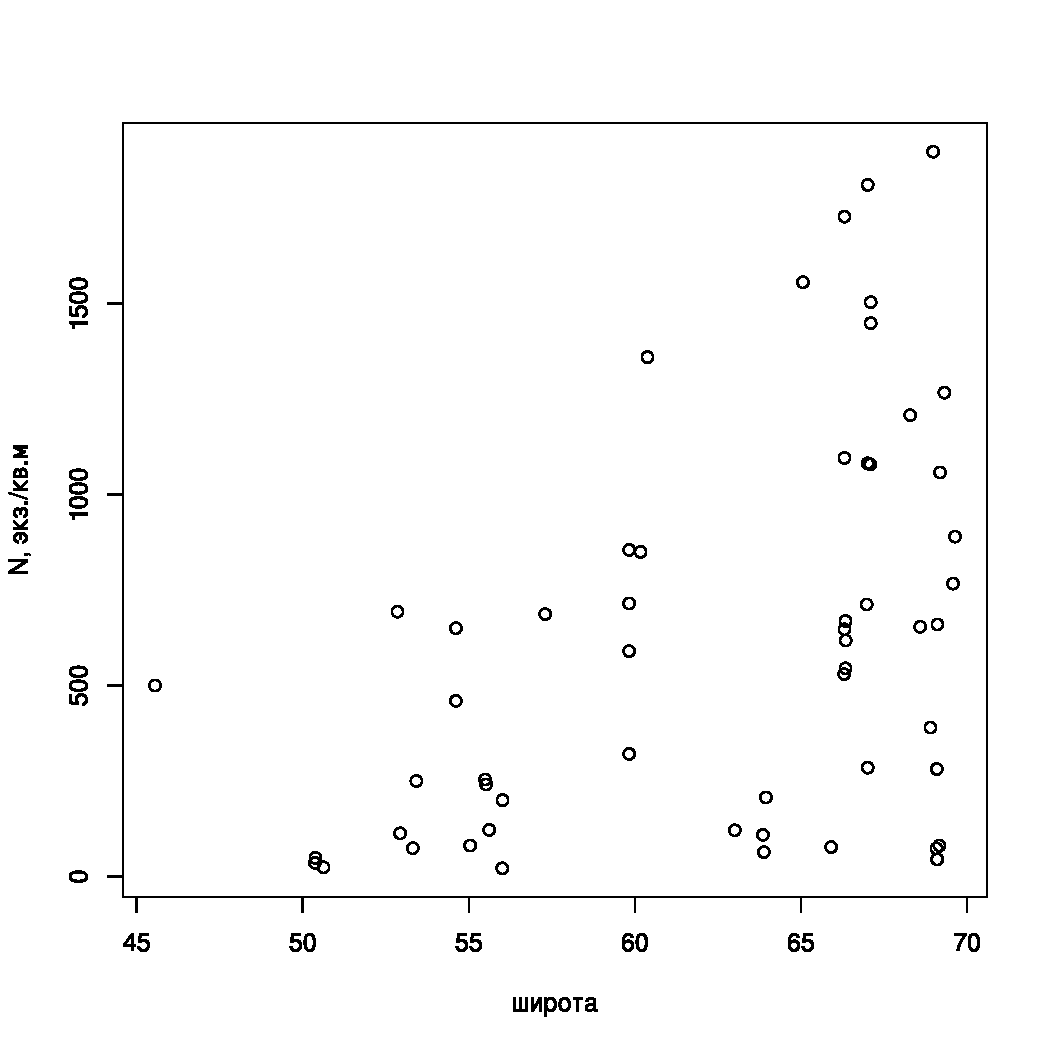
\includegraphics[width=\textwidth]{../macrodistribution/lat_vs_Nmean1.pdf}
    \caption{Изменение численности {\it Macoma balthica} с географической широтой}

{\footnotesize Примечание: N~--- средняя численность {\it M.~balthica},~экз./м$^2$}
    \label{ris:lat_vs_Nmean}
	\end{figure}
Возможно, более показательно рассматривать максимальные средние значения, поскольку они показывают, какого максимального значения может достигать обилие в данном регионе.
По данным, представленным на рисунке \ref{ris:lat_vs_Nmean}, видно, что максимальная средняя численность маком монотонно увеличивается с широтой.
Таким образом, распределение вида {\it M.~balthica} в европейской части ареала может быть описано как увеличивающееся к северу (<<ramped north>>) (\cite{Sagarin_Gaines_2002}).

Максимальные средние численности маком в пределах европейской части ареала отмечены для Белого и Балтийского морей (рис.~\ref{app:NB_areal}).
Интересно, что оба этих водоема характеризуются пониженной соленостью (\cite{Dobrovolskiy_Zalogin_1982}).
Возможно, в условиях пониженной солености конкуренция оказывается ниже, за счет исчезновения более стеногалинных видов, и макома может достигать большего обилия.
Также на обилие может влиять доступность пищевых ресурсов. 
Такой эффект известен при сравнении условий обитания в отдельных поселениях.
Л.~Басовой для Кольского залива была показана достоверная положительная корреляция между численностью {\it M.~balthica} и содержанием органических веществ в грунте (\cite{Basova_2004}).   
Мы не обнаружили подобной закономерности, в то же время, по нашим данным, численность маком достоверно коррелировала с долей песчаный фракций. 
Была показана прямая связь с мелким песком и обратная~--- с крупным (табл.~\ref{tab:grunt_N_correlation_Barents}).
Обычно предполагается, что предпочтение особями более мелкодисперсных грунтов связано с более высокой концентрацией органических веществ в таком грунте. 
Хотя часто концентрация органических веществ положительно коррелирует с долей мелкого песка и алевро-пелита (\cite{Bubnova_1972, Basova_2004}), для исследованных участков на статистическом уровне этого не показано, хотя и наблюдается тенденция к этому. 
Показано (\cite{Olafsson_1989}), что на песчаном грунте {\it M.~balthica} начинают питаться не как собирающие детритофаги, а как фильтраторы. 
Таким образом, основную роль начинают играть не органические вещества в осадках, растворенные в воде. 
В таком случае наличие в Кольском заливе поселков и городов, в которых есть бытовые стоки, может объяснять более высокое обилие маком именно в данной акватории.

%Написать что-то про продуктивность Белого и Балтийского моря. Возможно сравнить их с тем же Северным. Понять только по какому параметру. Прямая органика. Планктон???

Для сравнения оценок биомассы моллюсков {\it M.~balthica}, полученных в ходе данного исследования, с данными по европейской части ареала была собрана опубликованная информация о средней биомассе особей {\it M.~balthica} в различных акваториях (прил.~\ref{app:NB_areal}).
Мы использовали данные о биомассе, измеренной как суммарный сырой вес особей в поселении.
Для того чтобы расширить географию наблюдений, данные о сухом весе и беззольном сухом весе были пересчитаны в сырой вес с использованием пересчетных коэффициентов (\cite{Ricciardi_Bourget_1998}).
Максимальная биомасса была отмечена в центральной части ареала~--- в Северном и Балтийском морях (рис.~\ref{ris:B_macrodistribution}).
	\begin{figure}[p]
    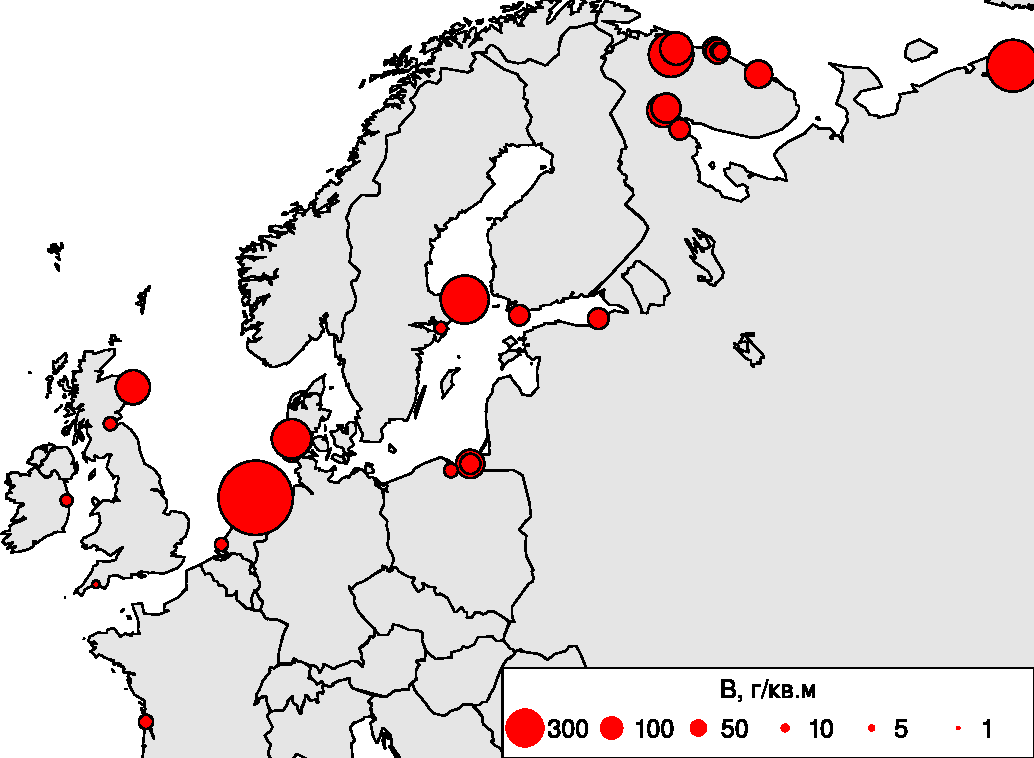
\includegraphics[width=\textwidth]{../macrodistribution/Bmean_ru1.pdf}
    \caption{Биомасса {\it Macoma balthica} в европейской части ареала}

{\footnotesize Примечание: Площадь кругов пропорциональна средней биомасса (B) моллюсков,~г/м$^2$ \\
Источники данных см. в прил.~\ref{app:NB_areal}.}
    \label{ris:B_macrodistribution}
	\end{figure}
На южном краю ареала биомасса ожидаемо снижается, в то время как в северной части ареала биомасса сравнима со средними значениями в центральной части ареала, хотя и не достигает максимальных.
Таким образом, распределение поселений с различной биомассой в целом соответствует гипотезе об обилии в центре (\cite{Sagarin_Gaines_2002}).


\afterpage{\clearpage}

%%%%%%%%%%%%%%%%%%%%%%%%%%%%%%%%%
%структура поселений маком.
	\subsection{Особенности структуры поселений {\it Macoma balthica}}
Для \textit{M.~balthica} описано бимодальное и мономодальное распределение особей (\cite{Segerstrale_1969, Maximovich_et_al_1991, Nikolaeva_1997, Nikolaeva_1998}). 
При массовом оседании личинок  \textit{M.~balthica}, в зависимости от выживаемости сеголеток, возможно два варианта развития поселения. 
Если выживаемость хорошая, то можно наблюдать ежегодное смещение модального класса по оси размеров. 
При новом оседании личинок до полного отмирания особей первой генерации формируется бимодальное распределение. 
Другой описанный вариант~--- к следующему сезону сеголетки практически исчезают, и происходит новое оседание личинок. 
При повторении этой схемы наблюдается мономодальное распределение с доминированием по численности самых мелких особей (сеголеток) при практически полном отсутствии крупных особей. Естественно, при плохой выживаемости и отсутствии значительного оседания личинок поселение достаточно быстро отмирает (\cite{Maximovich_et_al_1991}).

В исследованных нами поселениях размерная структура \textit{M.~balthica} значительно варьирует, однако при достаточно высокой численности моллюсков мы наблюдаем две наиболее характерные ситуации: мономодальное распределение особей по размерам чаще всего с преобладанием молодых особей, и бимодальное распределение.

Рассматривая динамику размерной структуры, можно говорить о  двух ситуациях, которые мы наблюдали в исследованных поселениях.
Наиболее распространена ситуация, в которой наблюдается смена типа структуры со временем. 
Сначала в поселении наблюдается мономодальная структура с преобладанием относительно молодых, и со временем мы можем наблюдать смещение модального класса по оси размеров. 
Через несколько лет происходит следующее успешное пополнение поселения молодью и формируется бимодальное распределение.
Со временем происходит элиминация старших особей и, в зависимости от периода через который происходит следующее успешное пополнение поселения молодью, мы либо продолжаем наблюдать бимодальное распределение, либо оно вновь становится мономодальным.
Такой тип динамики отмечен нами для всех поселений в районе Лувеньгских шхер, Западной Ряшковой салмы (прил.~\ref{app:White_sizestr_hist}) и для Дальнего пляжа губы Дальне-Зеленецкая (прил.~\ref{app:Barents_sizestr_hist}).
Подобная картина была ранее описана для Сухой салмы в губе Чупа Белого моря (\cite{Maximovich_et_al_1991}).
В Балтийском море описан аналогичный тип динамики (\cite{Segerstrale_1969}).

Другой вариант динамики размерной структуры, по-видимому, менее распространен.
Он выглядит как ежегодное повторение мономодальной размерной структуры в течение нескольких лет.
Такой вариант был описан для поселений \textit{M.~balthica} в Южной губе о.~Ряшкова и на о.~Ломнишном (прил.~\ref{app:White_sizestr_hist}).
Интересно отметить, что оба поселения находились под влиянием хищной улитки \textit{Amauropsis islandica} (\cite{Aristov_Granovich_2011}).
Однако для того чтобы аргументированно говорить о влиянии хищников, необходимы отдельные исследования.
Сходный тип динамики был описан для бухты Клющиха в губе Чупа Белого моря (\cite{Maximovich_et_al_1991, Gerasimova_Maximovich_2013}.
Все участки, на которых описан подобный тип развития поселения, сходны по топическим условиям~--- песчаный пляж с минимальным заилением.
Это подтверждает предположение, высказанное ранее (\cite{Gerasimova_Maximovich_2013}), что возможность формирования такого типа динамики может быть связана с расхождением по типу питания у молодых и взрослых маком.
Для Балтийского моря было показано, что на илисто-песчаном грунте и взрослые, и молодые моллюски питаются как собирающие детритофаги, в то время как на песчаном грунте, в условиях активной гидродинамики, где молодь питаются как собирающие детритофаги, а взрослые~--- как фильтраторы (\cite{Olafsson_1989}). 
Аналогичное различие в пищевом поведении было показано и для Белого моря (\cite{Gerasimova_1988}).

\afterpage{\clearpage}

%%%%%%%%%%%%%%%%%%%%%%%%%%%%%%%%%
		\section{Скорость роста {\it Macoma balthica} как отражение условий обитания}
% скорость роста как показатель "условий жизни"

% MSc discussion
Закономерности линейного роста двустворчатых моллюсков неоднократно являлись предметом специальных исследований. При этом  с одной стороны рассматривают различия в ростовых характеристиках моллюсков одного вида в разных поселениях, а с другой анализируют неоднородность в характере роста особей в пределах локального местообитания (например, \cite{Segerstrale_1960, Beukema_et_al_1977, Thompson_Bayne_1974, Jensen_1993, Grant_Thorpe_1991}). 

Известно, что на скорость роста влияют условия питания (\cite{Beukema_Meehan_1985, Thompson_Nichols_1988}).
Поскольку время питания зависит от осушки, для Баренцева моря было проведено сравнение ростовых характеристик по горизонтам литорали. Однако выделяющиеся группы не были связаны с мареографическим уровнем.

Межгодовые различия в условиях обитания (например, масштабные температурные и соленостные колебания, характерные для Баренцева моря (Терещенко, 1997) могут вносить значительный шум в наблюдаемую картину сравнений темпов роста. 
Для того, чтобы снять их влияние, необходимо проанализировать рост особей из одной или максимально близких генераций. 
Однако, при анализе особей старше 8 лет наблюдаемая картина не отличалась от сравнения тотальных выборок.

Для ряда видов Bivalvia отмечалось определяющее влияние стартовых (ко второму сезону роста) средних размеров моллюсков на темп их роста впоследствии (в течение всего жизненного цикла). 
Так, это было показано для {\it Macoma incongrua}  в Японском море (\cite{Maximovich_Lysenko_1986}), {\it Mytilus trossulus septentrionalis} в Чаунской губе Восточно-Сибирского моря (\cite{Gagaev_et_al_1994}) и {\it Mytilus edulis} в Кандалакшском заливе (\cite{Maximovich_et_al_1993}). 
Для {\it M.~balthica} аналогичная зависимость было показана на поселениях в заливе Сан-Франциско (\cite{Cloern_Nichols_1978}). 

По нашим данным, стартовый размер особи оказывал достоверное влияние на годовой прирост, однако с увеличением стартового размера годовой прирост изменялся немонотонно — максимум приходился на стартовый размер $6-9$~мм. 
Таким образом, можно говорить об $S$-образном характере роста  {\it M.~balthica}, что характерно для живых организмов.
Более высокие значения годового прироста на нижнем горизонте литорали скорее всего связаны с условиями питания: при меньшей осушке время питания увеличивается.
Поскольку географический градиент запад-восток оказался связан с увеличением размера частиц грунта, возможно, что именно гранулометрический состав грунта влияет на годовой прирост. 

% про методы сравнения роста - сравнение коэффициентов Берталанфи


% сравнение кривых роста по Максимовичу


%скорость роста в разных частях ареала. Букма-Меган - врисовать наши точки в их картинку...
\afterpage{\clearpage}

\par\bigskip

В рамках анализа полученных нами данных по росту маком в Баренцевом море, мы провели анализ широтных изменений параметра $\omega$ с использованием доступных литературных источников, добавив работы по российской части Балтийского моря и данные по Белому морю (рис.~\ref{ris:omega_vs_lat}).
	\begin{figure}[p]
	\begin{center}	
		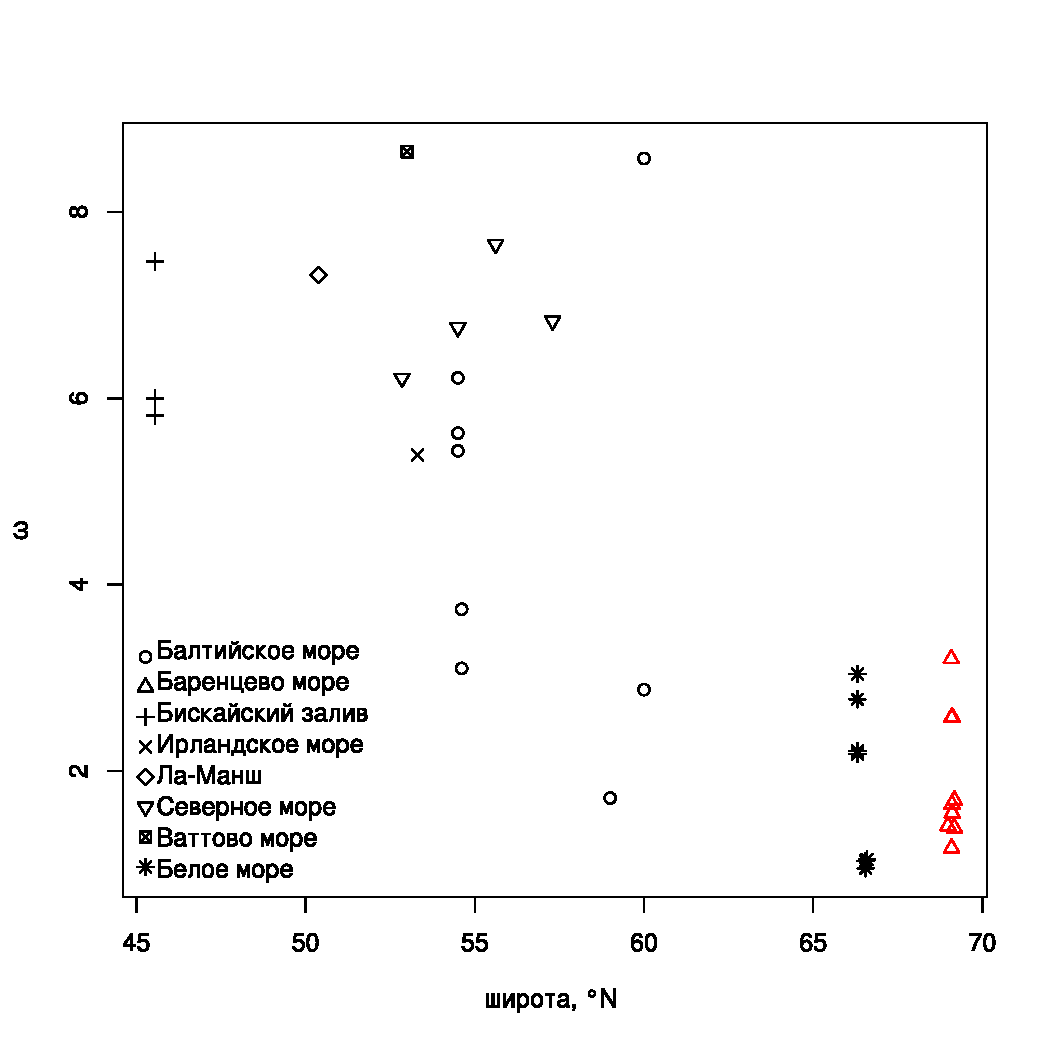
\includegraphics[width=\textwidth]{../Growth_sravnenie/long_vs_omega_ru.pdf}
	\end{center}
		\caption{Широтное изменение ростовых характеристик {\it M.~balthica} в европейской части ареала}

	\footnotesize{Примечание: $\omega = L_{\infty} \times k$, где $L_{\infty}$ и $k$~--- коэффициенты уравнения роста Берталанфи.\\ 
	Источники см. в приложении \ref{app:growth_omega}}
		\label{ris:omega_vs_lat}
	\end{figure}
Наши данные подтверждают гипотезу о снижении скорости роста в северных частях ареала маком (корреляция Спирмена: $r_{s} = -0,60$, $p < 0,0001$).

Однако, в Балтийском море присутствуют поселения со скоростью роста, сравнимыми с характеристиками для арктических морей~--- Белого и Баренцева (рис.~\ref{ris:omega_vs_lat}). 
По-видимому, это связано с влиянием низкой солености на скорость роста (\cite{Segerstrale_1960, Kube_et_al_1996}).
Данные по Балтийскому морю наиболее разнородны: параметр $\omega$ варьирует от $1,7$ до $8,6$ (приложение~\ref{app:growth_omega}), при этом даже оценки для одного района, данные разными исследователями, могут значительно отличаться.


Для учета варьирования реальных ростовых характеристик мы сравнили имеющиеся в литературе данные и полученные нами данные с учетом разброса эмпирических данных относительно регрессионной модели.
Всего было использовано $33$ описания с $23$ географических точек на Европейском побережье Северной Атлантики (приложение~\ref{app:growth_sources}).
Мы использовали данные о первых $6$ годах роста особей, для унификации длины сравниваемых рядов.
Было выделено $6$ групп моллюсков, различающихся по ростовым характеристикам (рис.~\ref{ris:growth_cluster_literature}).
	\begin{figure}[p]
	\begin{center}	
		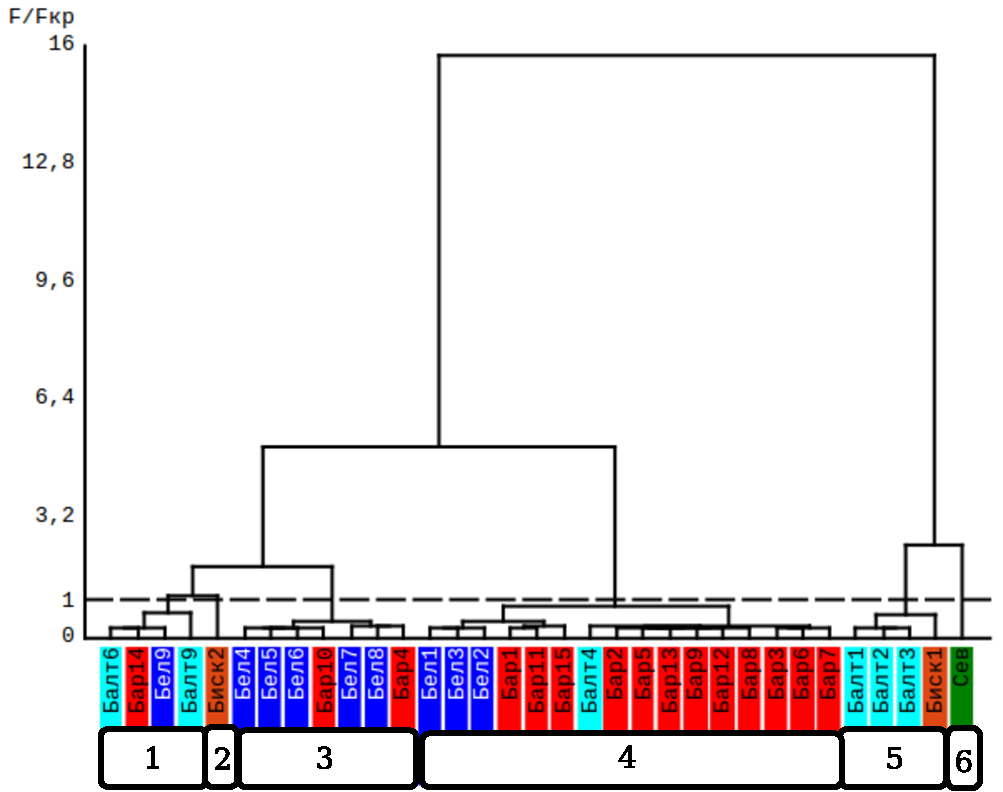
\includegraphics[width=\textwidth]{../Growth_sravnenie/Europe_clusters_usrednenie.pdf}
	\end{center}
		\caption{Классификация поселений маком на Европейском побережье в Северной Атлантике по моделям линейного роста}


	\footnotesize{Примечание: Дендрограмма сходства 33 рядов, аппроксимированных уравнением Берталанфи. 
Способ объединения рядов в кластеры~--- усреднение значений переменной $Y$, соответствующих одному значению $X$.
Мера сходства~--- $F/F_{kp}$ (уровень значимости $\alpha = 0,05$)

Обозначения поселений указаны в приложении~\ref{app:growth_sources} \\
Цвета: Красный~--- Баренцево море, синий~--- Белое море, голубой~--- Балтийское море, зеленый~--- Северное море, оранжевый~--- Бискайский залив}
		\label{ris:growth_cluster_literature}
	\end{figure}

Максимальная скорость роста была отмечена для группы $6$ (рис.~\ref{ris:growth_model_europe})~--- поселение в Северном море (\cite{Vogel_1959}). 
	\begin{figure}[p]
	\begin{center}	
		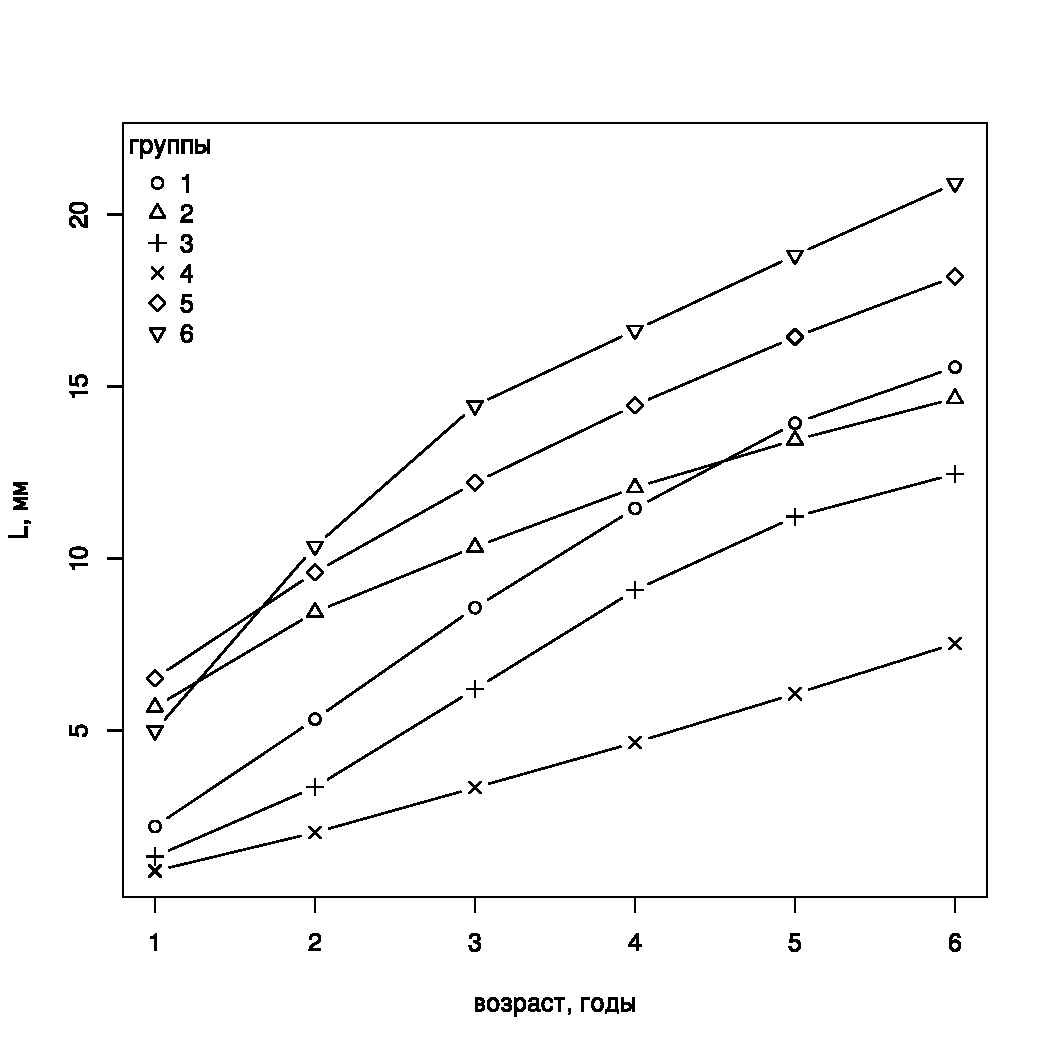
\includegraphics[width=\textwidth]{../Growth_sravnenie/Europe_growth_groups1.pdf}
	\end{center}
		\caption{Модели роста, передающие принципиальные свойства вариации характера линейного роста маком в Европейской части ареала}

	\footnotesize{Примечание: L, мм~--- длина раковины. Номера групп в легенде соответствуют рис.~\ref{ris:growth_cluster_literature})}
		\label{ris:growth_model_europe}
	\end{figure}
Группа $4$, в которую вошло большинство изученных нами поселений в Баренцевом море, характеризуется минимальной скоростью роста.
Также в эту группу вошла часть Беломорских поселений (\cite{Semenova_1970}) и одно поселение в Балтийском море (\cite{Bergh_1974}).
Часть исследованных поселений в Баренцевом море отличалась более высокой скоростью роста, и попала в группы $3$ (<<Беломорский>> кластер) и $1$ (Беломорские, Балтийские и Баренцевоморские поселения).
Интересно отметить, что более южные поселения (входящие в состав групп $2$ и $5$~--- <<Балтийский>> кластер), в Бискайском заливе (\cite{Bachelet_1980}), характеризуются более низкой скоростью роста , чем в центральной части ареала (рис.~\ref{ris:growth_model_europe}).
Данный результат хорошо согласуется с <<гипотезой об обилии в центре>> (<<abindant-centre hypothesis>>, \cite{Sagarin_et_al_2006}) и ранее проведенными исследованиями (\cite{Beukema_Meehan_1985, Hummel_et_al_1998}).

\afterpage{\clearpage}

%%%%%%%%%%%%%%%%%%%%%%%%%%%%%%%%%
%динамика поселений
\section{Долговременные тренды в поселениях \textit{Macoma~balthica}}


	\subsection{Анализ динамики численности {\it Macoma balthica} в Кандалакшском заливе Белого моря}
При изучении динамики численности можно анализировать несколько компонентов.
Первый компонент --- наличие или отсутсвие тренда как направленноого изменения численности.
При убирании тренда остается компонент динамики, для которого двумя крайими случаями будет: стабильная численность, которая поддерживается за счет плотностнозависимых процессов как систем обраной связи и неконтролируемый рост численности популяции по экспоненте.

Мы проанализировали динамику численности {\it M.~balthica} на каждом участке на наличие тренда при помощи теста Мантеля (табл.~\ref{tab:Mantel_N2_trend}).
	\begin{table}[ht]
	\caption{Выявление трендов в динамике численности {\it Macoma balthica} на различных участках Белого моря.}
	\label{tab:Mantel_N2_trend}
        \begin{tabular}{|p{0.25\textwidth}|*{2}{p{0.2\textwidth}|p{0.25\textwidth}|}} \hline
	Участок & $Mantel$ & $p$ & наличие тренда
	\\ \hline
	Эстуарий р. Лувеньга & 0,3168 & 0,003 & есть
	\\ \hline
	о. Горелый & 0,0269 & 0,368 & нет
	\\ \hline
	материковая литораль (Лувеньга) & 0,6103 & 0,001 & есть
	\\ \hline
	Южная губа о. Ряшков & 0,3687 & 0,015 & есть
	\\ \hline
	Запдная Ряшкова салма & 0,0108 & 0,404 & нет
	\\ \hline
	Ломнишный & -0,0999 & 0,47 & нет
	\\ \hline
	г. Медвежья & 0,0154 & 0,385 & нет
	\\ \hline
	г. Сельдяная & 0,2524 & 0,003 & есть
	\\ \hline
	\end{tabular}
	%    {\footnotesize Примечание: достоверность различий *** \textemdash $p<0,001$; ** \textemdash $p<0,05$; * \textemdash $p<0,1$.}
	\end{table}

Было показано наличие тренда на 4 участках: эстуарий р.~Лувеньга, материковая литораль в районе пос. Лувеньга, Южная губа о.~Ряшкова, г. Сельдяная.
Для удаления тренда из исходных значений были вычтены предсказанные значения из регрессионной модели $N = a + b*T$, где $N$ --- численность, экз./м$^2$, $T$ --- годы.
По детрендированному ряду были рассчитаны частные автокорреляции ($PRCF$ - partial rate correlation function).  
Коррелограммы представлены на рисунке \ref{ris:perm_PRCF_Kandalaksha_N2_detrend}.
	\begin{figure}[ht]
	
	\begin{minipage}[b]{.46\linewidth}
	%Фигурка в первом ряду слева размер отведенный под весь этот объект \textendash 0.46 от ширины строки
	%Параметр [b] означает, что выравнивание этих министраниц будет по нижнему краю
	\begin{center}
	{\footnotesize Эстуарий р.~Лувеньги}
		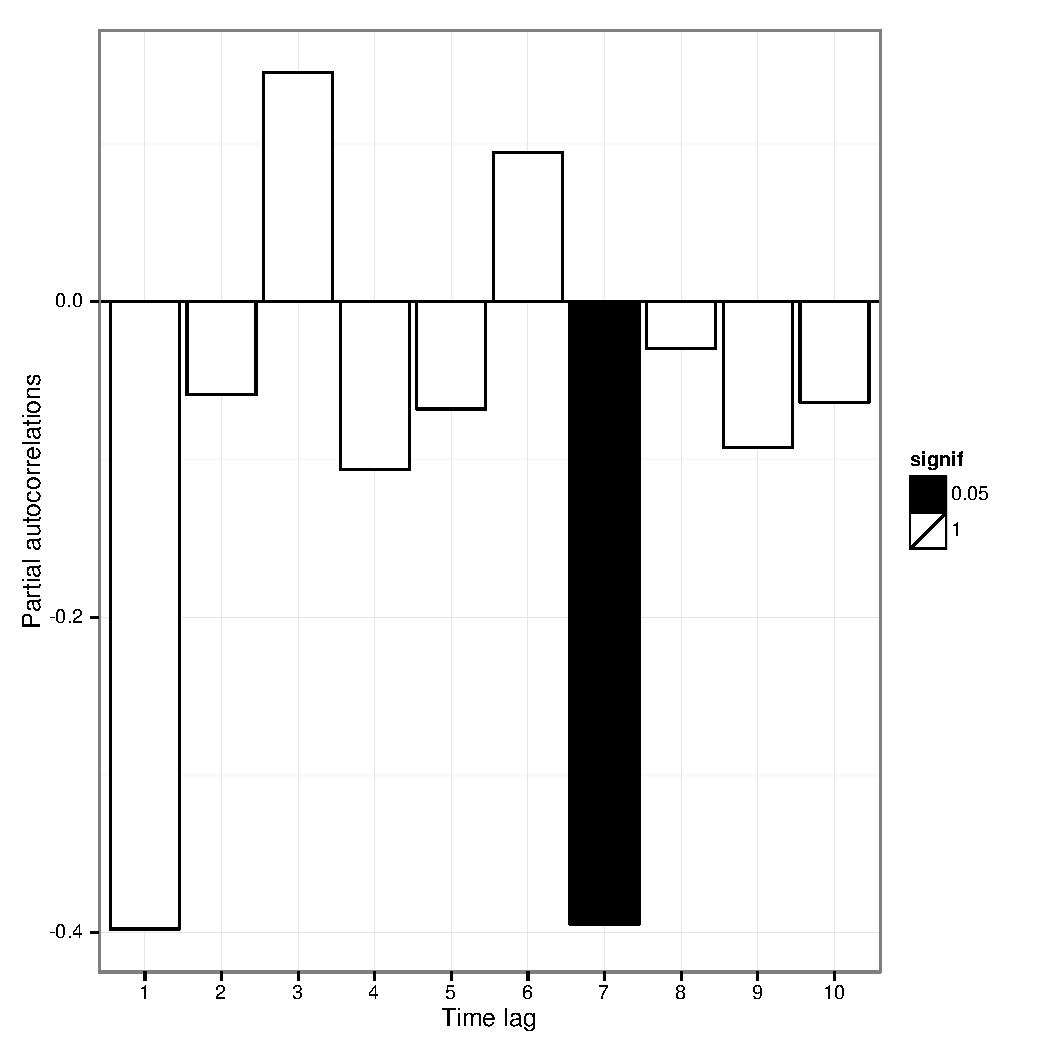
\includegraphics[width=65mm]{../White_Sea/dynamic_N_N1/perm_PRCF_Estuary_detrend.pdf}

	\end{center}
	\end{minipage}
		\hfil %Это пружинка отодвигающая рисунки друг от друга
	\begin{minipage}[b]{.46\linewidth}
%Следующий рисунок - первый ряд справа %DUNGEON S_4 \ AB
	\begin{center}
	{\footnotesize о.~Горелый}
		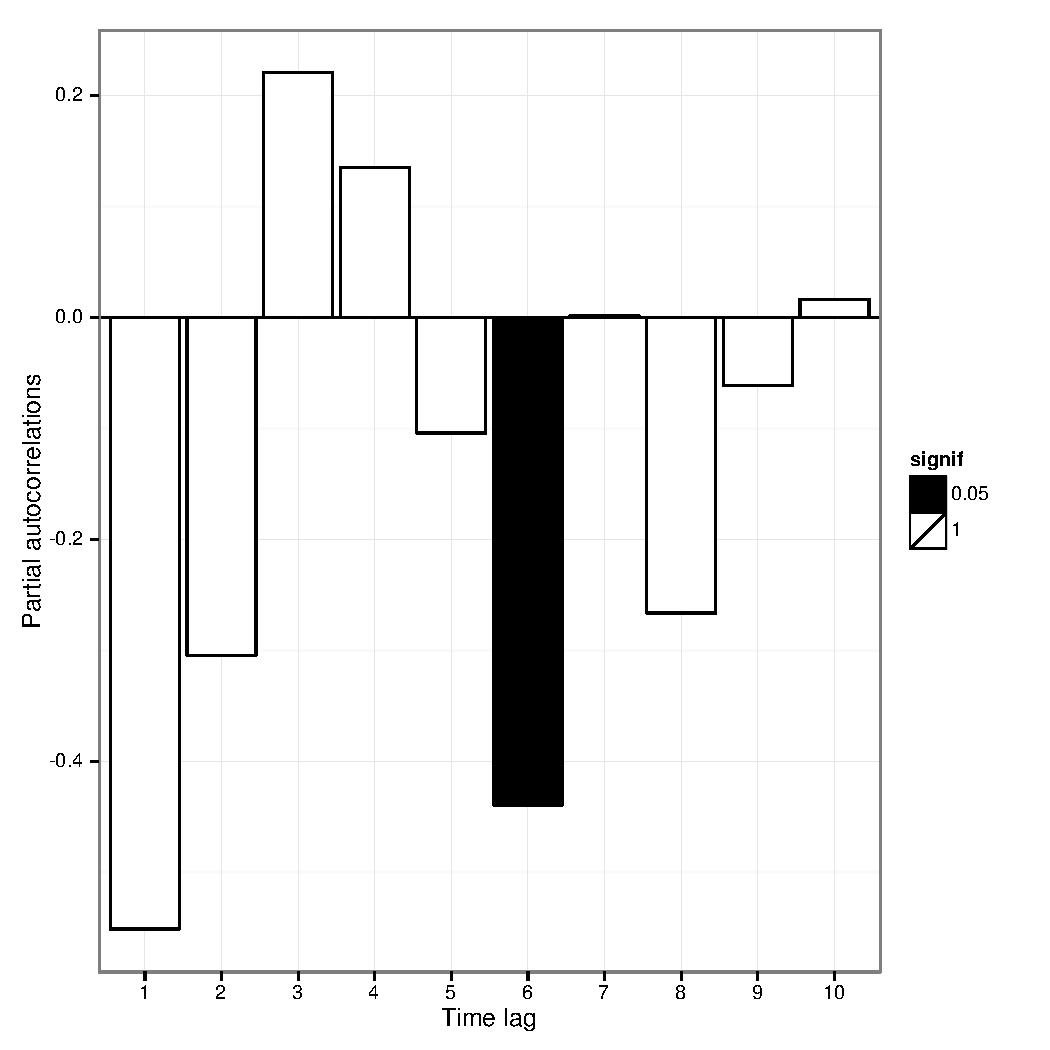
\includegraphics[width=65mm]{../White_Sea/dynamic_N_N1/perm_PRCF_Goreliy_all_detrend.pdf}
	\end{center}
	\end{minipage}

	\begin{minipage}[b]{.46\linewidth}
%Фигурка в первом ряду слева размер отведенный под весь этот объект \textendash 0.46 от ширины строки
%Параметр [b] означает, что выравнивание этих министраниц будет по нижнему краю
	\begin{center}
	{\footnotesize материковая литораль (Лувеньга)}
	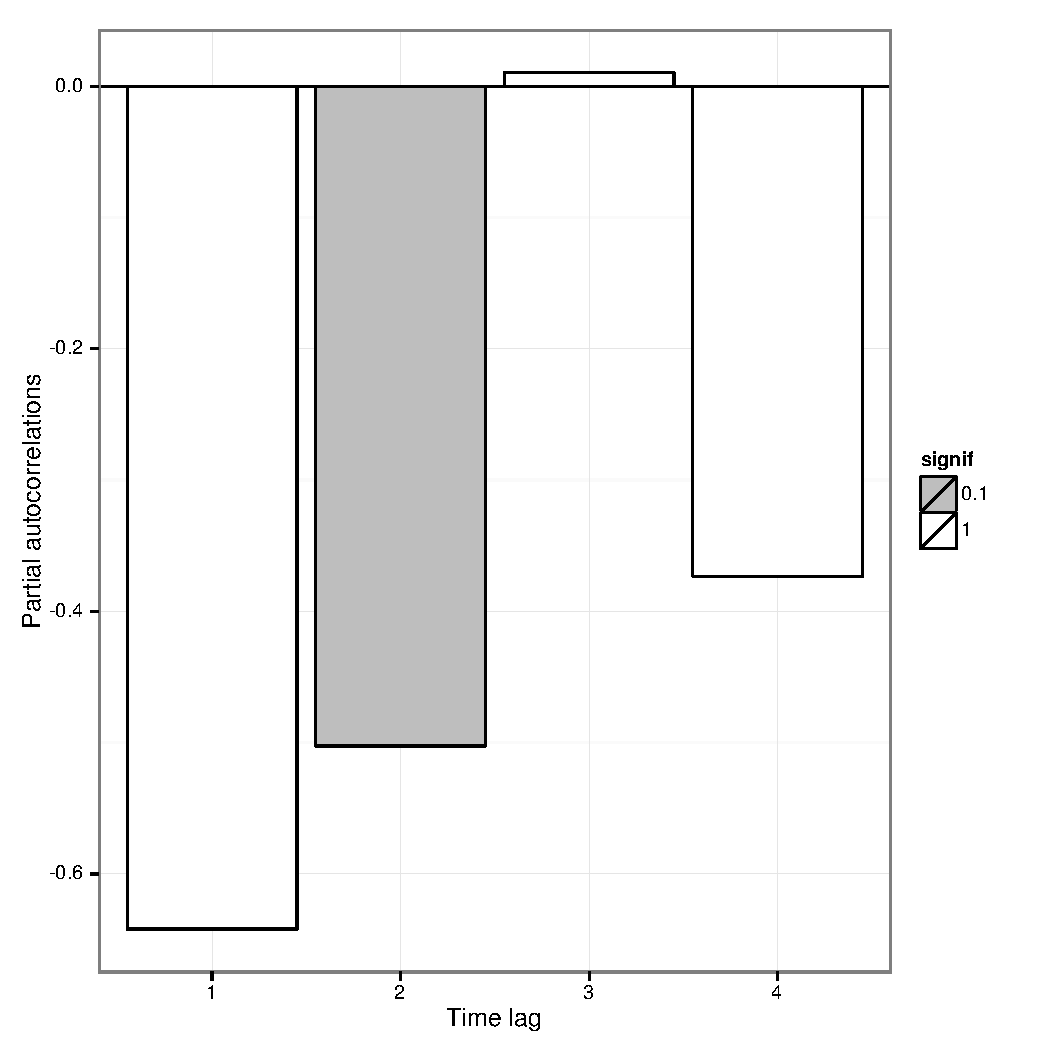
\includegraphics[width=65mm]{../White_Sea/dynamic_N_N1/perm_PRCF_razrez2_all_detrend.pdf}
	\end{center}
	\end{minipage}
		\hfil %Это пружинка отодвигающая рисунки друг от друга
	\begin{minipage}[b]{.46\linewidth}
%Следующий рисунок - первый ряд справа %DUNGEON S_4 \ AB
	\begin{center}
	{\footnotesize о.~Ломнишный}
	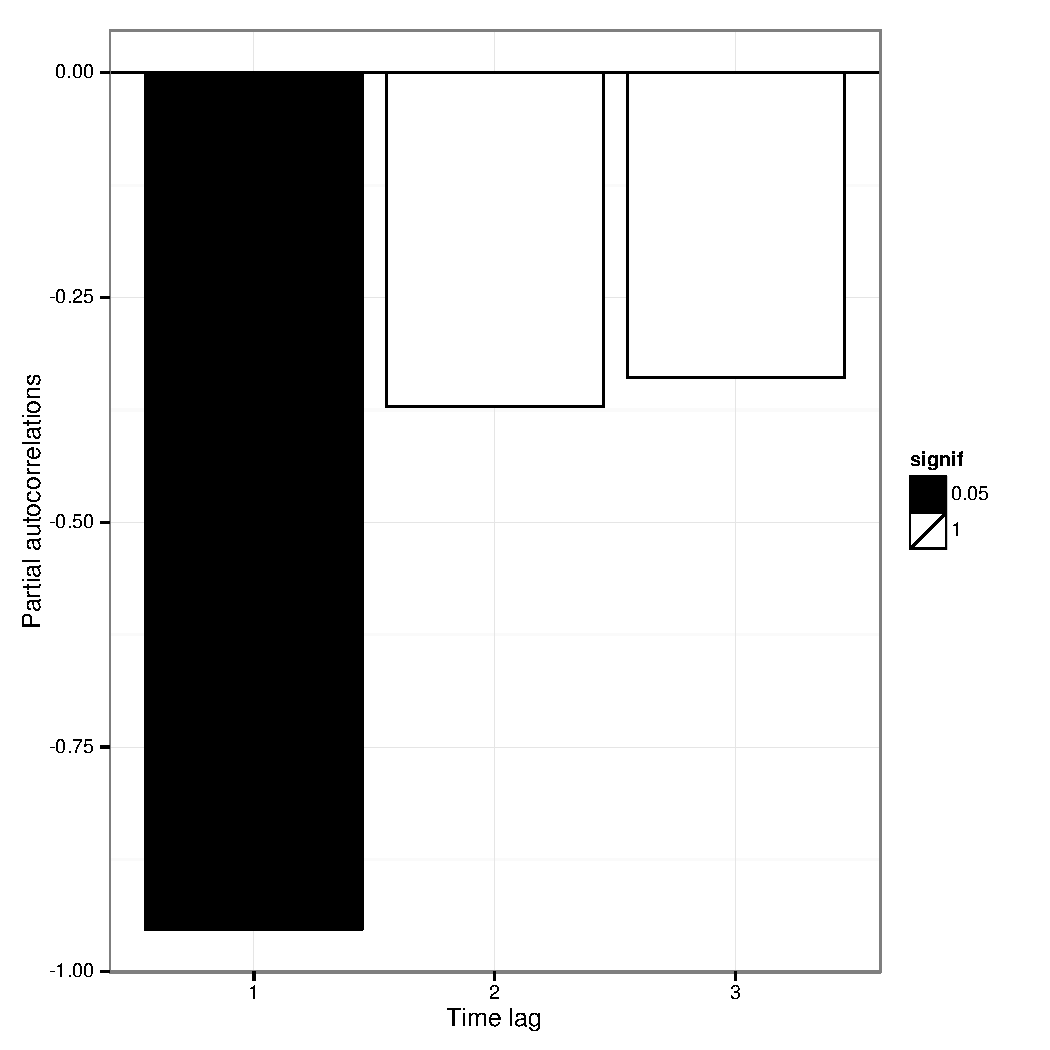
\includegraphics[width=65mm]{../White_Sea/dynamic_N_N1/perm_PRCF_Lomnishniy_detrend.pdf}
	\end{center}
	\end{minipage}

	\begin{minipage}[b]{.46\linewidth}
%Фигурка в первом ряду слева размер отведенный под весь этот объект \textendash 0.46 от ширины строки
%Параметр [b] означает, что выравнивание этих министраниц будет по нижнему краю
	\begin{center}
	{\footnotesize Южная губа о.~Ряшкова}
	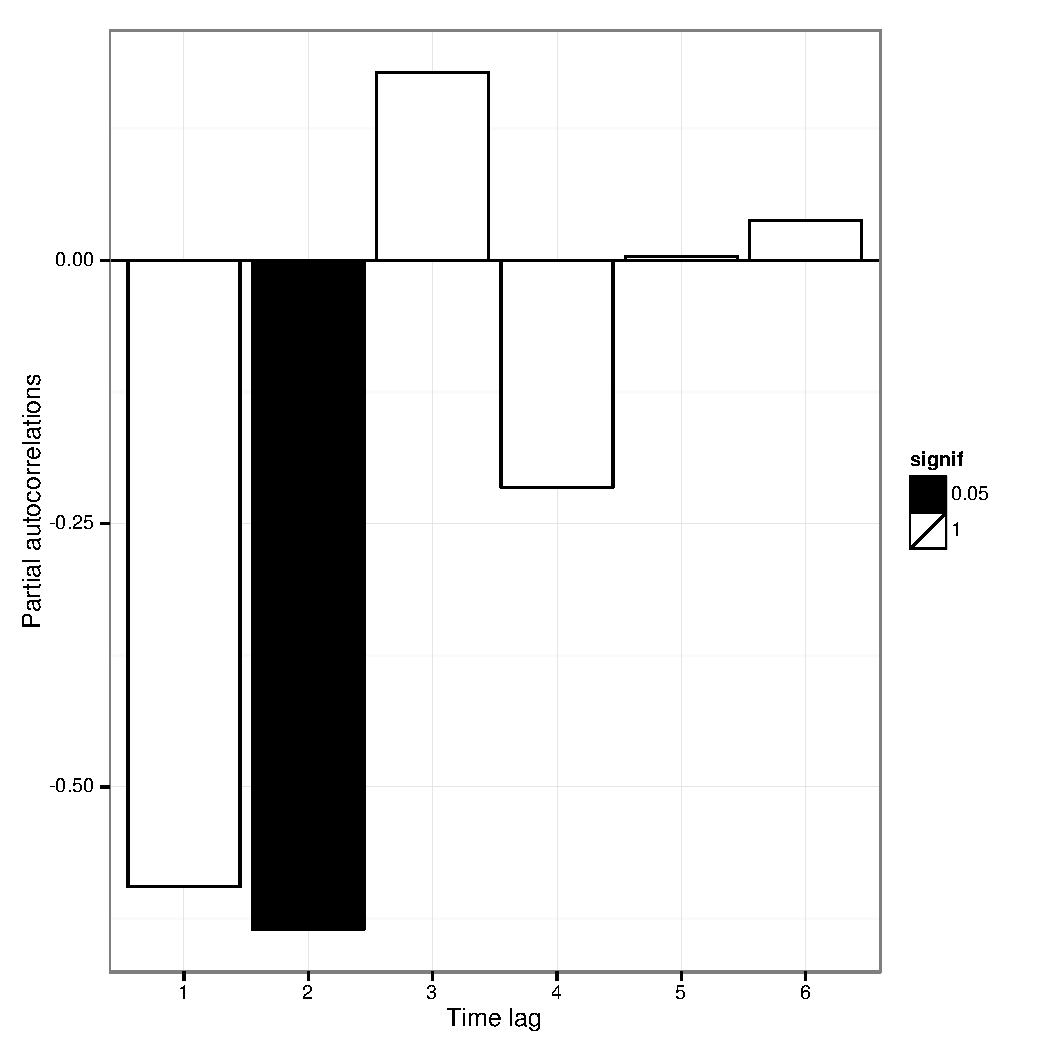
\includegraphics[width=65mm]{../White_Sea/dynamic_N_N1/perm_PRCF_YuG_detrend.pdf}
	\end{center}
	\end{minipage}
		\hfil %Это пружинка отодвигающая рисунки друг от друга
	\begin{minipage}[b]{.46\linewidth}
	\begin{center}	
	{\footnotesize Западная Ряшкова салма}
	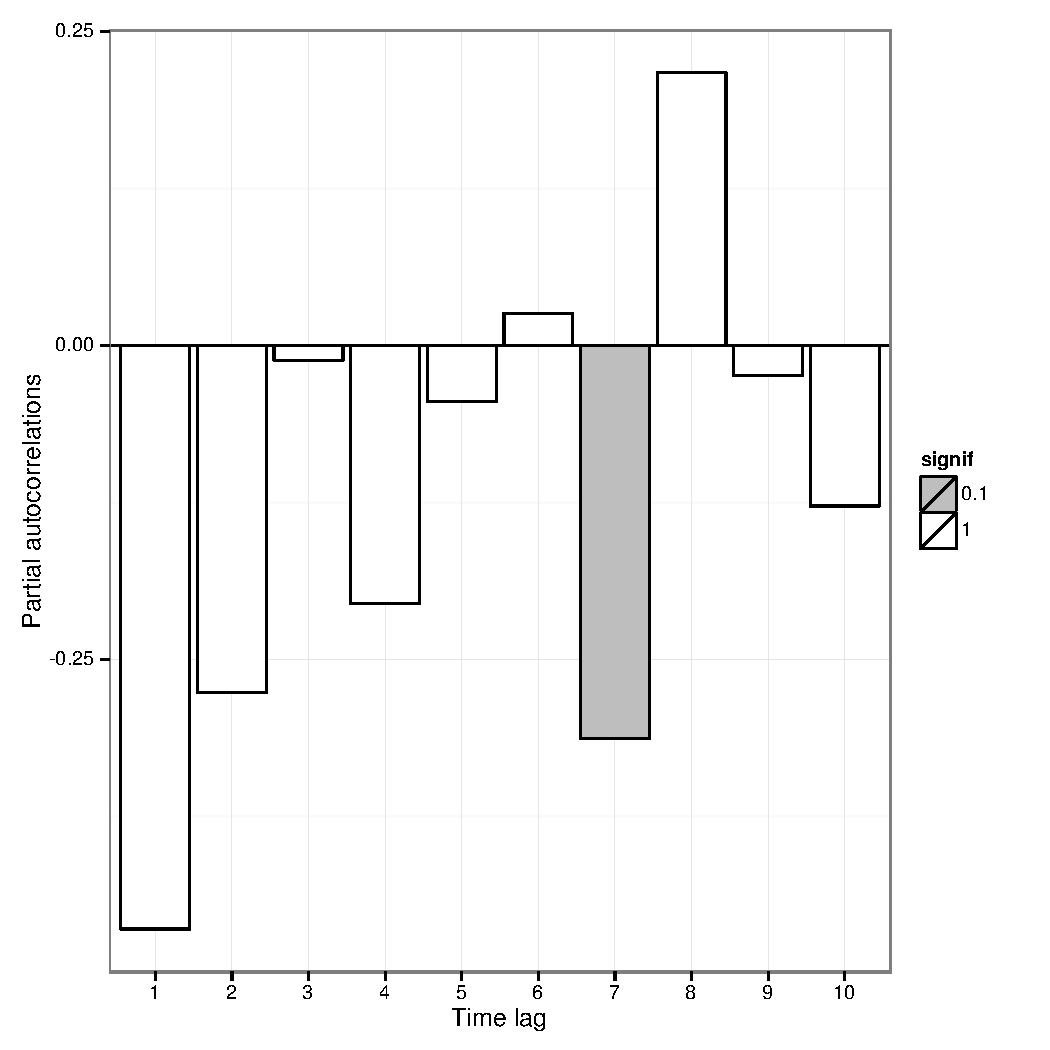
\includegraphics[width=65mm]{../White_Sea/dynamic_N_N1/perm_PRCF_ZRS_detrend.pdf}
	\end{center}
	\end{minipage}
	\caption{Частные корреляции численности {\it Macoma balthica} (без учета особей длиной менее 1 мм) в Кандалакшском заливе. Детрендированные данные. Оценка достоверности пермутационным методом.}
	\label{ris:perm_PRCF_Kandalaksha_N2_detrend}	
	\end{figure}

	\begin{figure}[ht]
%\smallskip

	\begin{minipage}[b]{.46\linewidth}
%Фигурка в первом ряду слева размер отведенный под весь этот объект \textendash 0.46 от ширины строки
%Параметр [b] означает, что выравнивание этих министраниц будет по нижнему краю
	\begin{center}
	{\tiny Медвежья}
	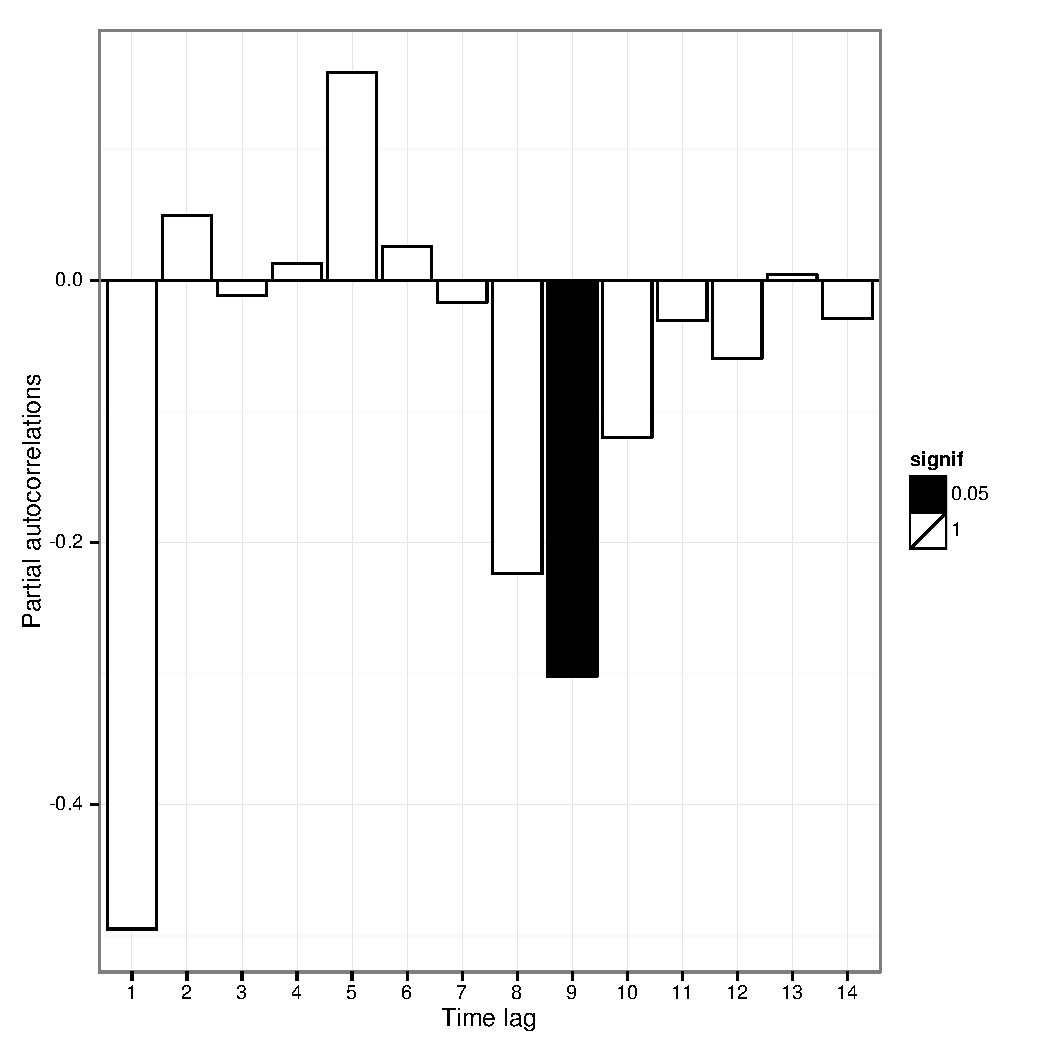
\includegraphics[width=65mm]{../White_Sea/dynamic_N_N1/perm_PRCF_Medvezhya_detrend.pdf}
	\end{center}
	\end{minipage}
%
	\hfil %Это пружинка отодвигающая рисунки друг от друга
%
	\begin{minipage}[b]{.46\linewidth}
	\begin{center}
	{\tiny Сельдяная}
	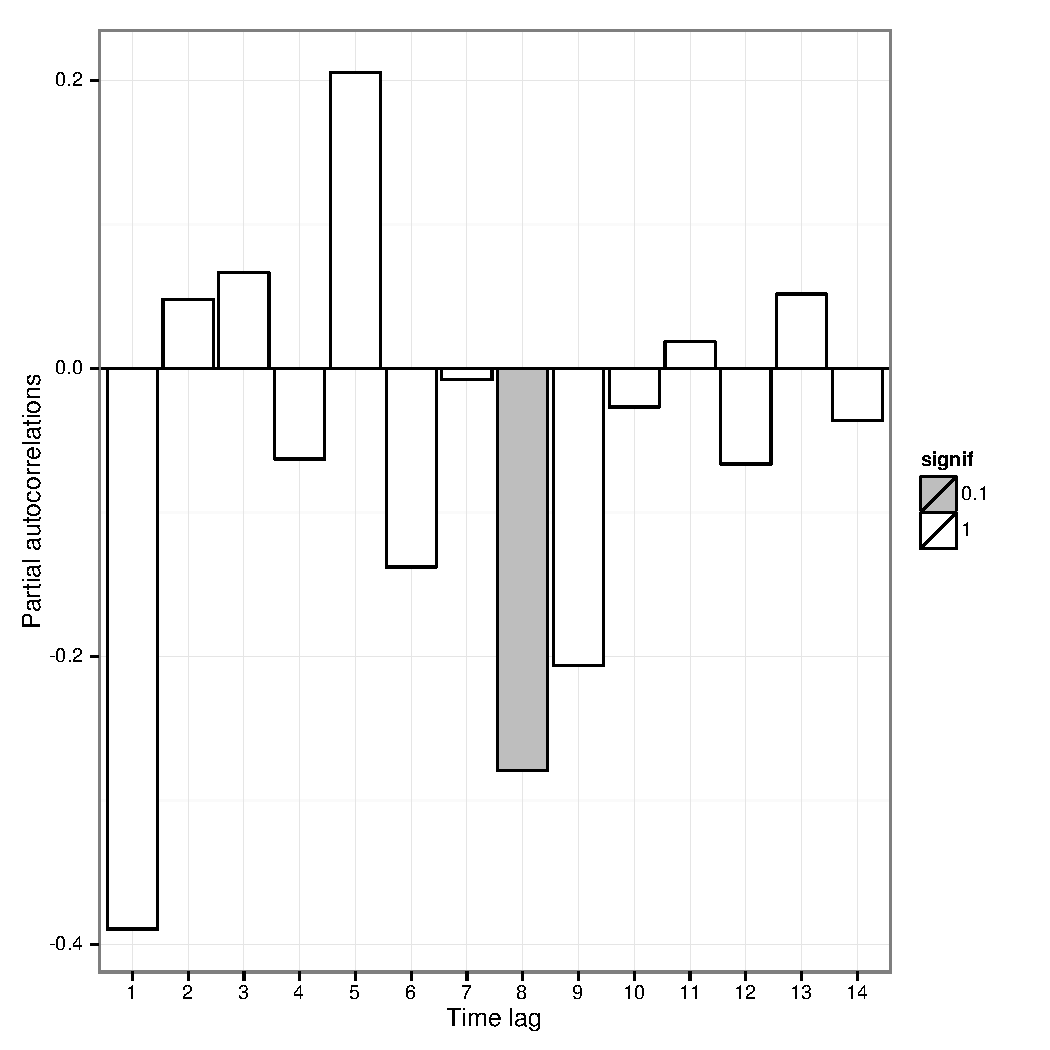
\includegraphics[width=65mm]{../White_Sea/dynamic_N_N1/perm_PRCF_Seldyanaya_detrend.pdf}
	\end{center}
	\end{minipage}

%\smallskip
%	\caption{Динамика плотности поселений {\it Macoma balthica} в вершине Кандалакшского залива}
%	\label{ris:dynamic_Kandalaksha_all}
\begin{center}
Рисунок \ref{ris:perm_PRCF_Kandalaksha_N2_detrend}, продолжение. Частные автокорреляции численности {\it Macoma balthica} (без учета особей длиной менее 1 мм) в Кандалакшском заливе. Детреднированные данные. Оценка достоверности пермутационным методом.
\end{center}
	\end{figure}
Для большинства временных рядов значение максимального значения достигает $PRCF$ с лагом 1, что характерно для динамики в отсутствие тренда. 
Достоверность частных автокорреляций оценивалась пермутационным методом.
Для участков в Южной губе о.~Ряшкова и на материковой литорали в Лувеньге были показаны достоверные значений $PRCF[2]$, причем в Южной губе $PRCF[2] > PRCF[1]$. 
Это показывает наличие в поселении плотностнозависимых процессов второго порядка.
Предположительно, это может быть воздействие хищников.
Мы надеемся проверить эту гипотезу в ходе дальнейших наблюдений.
Биологическая интерпретация $PRCF$ с большим лагом на настоящий момент представляется нам сомнительной.

		\subsection{Синхронность динамики численности {\it Macoma balthica} в Кандалакшском заливе Белого моря}
Для изучения синхронности колебаний численности маком мы использовали тест Мантеля.
Для включения большего количества рядов в анализ, он был проведен по двум наборам данных.
Первый набор данных включал участки, где при отборе проб промывка была на сите с диаметром ячеи $0,5$~мм. 
Сюда вошли участки в эстуарии р.~Лувеньги, на материковой литорали в районе Лувеньги, на о.~Горелый, в Западной Ряшковой салме и в губах Медвежья и Сельдяная.
Результаты корреляционного анализа представлены в таблице \ref{tab:Mantel_dynamic_N}.
	\begin{table}[ht]
	\caption{Синхронность динамики численности {\it Macoma balthica}.}
	\label{tab:Mantel_dynamic_N}
        \begin{tabular}{|p{0.2\textwidth}|*{8}{p{0.08\textwidth}|}} \hline
	$Mantel r \setminus p_{perm}$ & [1] & [2] & [3] & [4] & [5] & [6] & [7] & [8]
    \\ \hline
	[1] эстуарий р.~Лувеньги & & \cellcolor{yellow}{$0,002$} & $0,989$ & \cellcolor{yellow}{$0,009$} & \cellcolor{yellow}{$0,001$} & $0,264$ & \cellcolor{yellow}{$0,018$} & $0,441$
	\\ \hline
	[2] о.~Горелый & \cellcolor{yellow}{$0,929$} & & $0,393$ & \cellcolor{yellow}{$0,014$} & \cellcolor{yellow}{$0,001$} & $0,388$ & $0,992$ & $0,089$
	\\ \hline
	[3] о.~Ломнишный & $-0,439$ & $-0,067$ & & $0,208$ & $NA$ & $0,79$ & $0,082$ & $0,399$
	\\ \hline
 	[4] г.~Медвежья & \cellcolor{yellow}{$0,821$} & \cellcolor{yellow}{$0,86$} & $-0,028$ & & \cellcolor{yellow}{$0,001$} & $0,184$ & $0,932$ & $0,441$
	\\ \hline
	[5] материковая литораль (Лувеньга) & \cellcolor{yellow}{$0,781$} & \cellcolor{yellow}{$0,784$} & $NA$ & \cellcolor{yellow}{$0,704$} & & \cellcolor{yellow}{$0,044$} & $NA$ & $0,123$
	\\ \hline
	[6] г.~Сельдяная & $0,089$ & $-0,009$ & $-0,303$ & $0,087$ & \cellcolor{yellow}{$0,364$} & & $0,763$ & $0,818$
	\\ \hline
	[7] Южная губа о.~Ряшкова & \cellcolor{yellow}{$0,427$} & $-0,309$ & $0,333$ & $-0,213$ & $NA$ & $-0,127$ & & $0,585$
	\\ \hline
	[7] Западная Ряшкова салма & $-0,045$ & $0,057$ & $0$ & $-0,05$ & $0,284$ & $-0,141$ & $-0,038$
	\\ \hline
	\end{tabular}
	   {\footnotesize Примечание: Нижняя половина таблицы --- значение теста Мантеля, верхняя половина --- уровень значимости, определенный пермутационным методом. \\
Желтым выделены значения с уровнем значимости $< 0,1$. \\
$NA$ --- ряды не пересекаются во времени.}
	\end{table}
Три участка в районе Лувеньгских шхер (эстуарий р.~Лувеньги, о.~Горелый, материковая литораль) демонстрировали синхронную динамику поселений.
С данными участками была синхронна динамика поселения маком в г.~Медвежья. 
Низкая, хотя и достоверная корреляция была показана между динамикой на материковой литорали в районе Лувеньги и в г.~Сельдяной ($0,36$) и между эстуарием р.~Лувеньги и Южной губой о.~Ряшкова ($0,43$).


Второй набор данных включал участки, где при отборе проб промывку проводили на сите с диаметром ячеи $1$~мм.
Также сюда вошли те участки из предыдущего набора данных, где была известна размерная структура моллюсков --- из общей численности были вычтены численность особей длиной менее $1$~мм для возмодности сравнения.
Всего в данный анализ вошло 8 рядов данных: эстуарий р.~Лувеньги, материковая литораль в районе Лувеньги, о.~Горелый, Западная Ряшкова салма, Южная губа о.~ Ряшкова, о.~Ломнишный, б.~Клющиха и Сухая салма (табл.~\ref{tab:Mantel_dynamic_N2}).
	\begin{table}[ht]
	\caption{Синхронность динамики численности {\it Macoma balthica}.}
	\label{tab:Mantel_dynamic_N2}
        \begin{tabular}{|p{0.2\textwidth}|*{8}{p{0.08\textwidth}|}} \hline
	$Mantel r \setminus p_{perm}$ & [1] & [2] & [3] & [4] & [5] & [6] & [7] & [8]
	\\ \hline
	[1] эстуарий р.~Лувеньги & & $0,082$ & $0,646$ & $0,995$ & \cellcolor{yellow}{$0,029$} & $0,482$ & \cellcolor{yellow}{$0,013$} & $0,19$
	\\ \hline
	[2] о.~Горелый & $0,176$ &  & $0,067$ & $0,73$ & \cellcolor{yellow}{$0,001$} & $0,261$ & $0,986$ & \cellcolor{yellow}{$0,001$}
	\\ \hline
	[3] б.~Клющиха & $-0,046$ & $0,52$ &  & $0,673$ & \cellcolor{yellow}{$0,034$} & $0,213$ & $0,062$ & $0,065$
	\\ \hline
	[4] о.~Ломнишный & $-0,451$ & $-0,181$ & $-0,22$ &  & $NA$ & $1$ & $0,088$ & $0,341$
	\\ \hline
	[5] материковая литораль (Лувеньга) & \cellcolor{yellow}{$0,32$} & \cellcolor{yellow}{$0,862$} & \cellcolor{yellow}{$0,577$} & $NA$ &  & $0,117$ & $NA$ & \cellcolor{yellow}{$0,006$}
	\\ \hline
	[6]Сухая салма & $-0,019$ & $0,067$ & $0,085$ & $-1$ & $0,443$ &  & $0,688$ & $0,314$
	\\ \hline
	[7] Южная губа о.~ Ряшкова & \cellcolor{yellow}{$0,419$} & $-0,332$ & $0,434$ & $0,333$ & $NA$ & $-0,243$ &  & $0,605$
	\\ \hline
	[8] Западная Ряшкова салма & $0,114$ & \cellcolor{yellow}{$0,86$} & $0,72$ & $0,093$ & \cellcolor{yellow}{$0,755$} & $0,088$ & $-0,048$ & 
	\\ \hline
	\end{tabular}
	   {\footnotesize Примечание: Нижняя половина таблицы --- значение теста Мантеля, верхняя половина --- уровень значимости, определенный пермутационным методом. \\
Желтым выделены значения с уровнем значимости $< 0,05$. \\
$NA$ --- ряды не пересекаются во времени.}
	\end{table}
Интересно отметить, что при редукции данных до численности особей длиной более $1$~мм картина меняется.
Без изменения остается синхронность динамик поселений маком на материковой литорали в Лувеньге c о.~Горелый и эстуарием р.~Лувеньги.
Такжесохранияется синхронность динамик численности в поселениях в эстуарии р.~Лувеньга и Южной губе о.~Ряшкова.
В то же время поселение в Западной Ряшковой салме, который в предыдущем анализе показывало асинхронность по сравнению с остальными участками, в данном случае демонстрирует синхронность с поселениями на о.~Горелый и материковой литорали в Лувеньге.
Также показана синхронность динамик поселений на материковой литорали в Лувеньге и в бухте Клющиха.

Мы использовали значение теста Мантеля как меру сходства рядов данных для тестирования гипотезы, что на более близкорасположенных участках динамика численности {\it Macoma balthica} более сходна.
Для этого по координатам участков была рассчитана матрица расстояний между участками (табл.~\ref{tab:distance_area_km}).
	\begin{table}[ht]
	\caption{Расстояние между исследованными участками литорали.}
	\label{tab:distance_area_km}
        \begin{tabular}{|p{0.3\textwidth}|*{10}{p{0.04\textwidth}|}} \hline
	 & [1] & [2] & [3] & [4] & [5] & [6] & [7] & [8] & [9] & [10]
	\\ \hline
	[1] материковая литораль (Лувеньга) & 0,0 &  &  &  &  &  &  &  &  & 
	\\ \cline{1-3}
	[2] о.~Горелый & 1,5 & 0,0 &  &  &  &  &  &  &  &  
	\\ \cline{1-4}
	[3]эстуарий р.~Лувеньги & 1,0 & 1,0 & 0,0 &  &  &  &  &  &  &  
	\\ \cline{1-5}
	[4] Южная губа о.~Ряшкова & 11,7 & 10,7 & 11,7 & 0,0 &  &  &  &  &  & 
	\\ \cline{1-6}
	[5] о.~Ломнишный & 13,5 & 12,9 & 13,8 & 3,7 & 0,0 &  &  &  &  &  
	\\ \cline{1-7}
	[6] Западная Ряшкова салма & 11,9 & 10,8 & 11,8 & 1,7 & 5,3 & 0,0 &  &  &  &  
	\\ \cline{1-8}
	[7] г.~Сельдяная & 93,6 & 94,0 & 94,5 & 87,8 & 84,1 & 89,3 & 0,0 &  &  &  
	\\ \cline{1-9}
	[8] г.~Медвежья & 91,9 & 92,4 & 92,8 & 86,1 & 82,4 & 87,6 & 1,7 & 0,0 &  &  
	\\ \cline{1-10}
	[9] Сухая салма & 97,1 & 97,5 & 97,9 & 91,2 & 87,6 & 92,7 & 3,5 & 5,1 & 0,0 &  
	\\ \hline
	[10] б.~Клющиха & 100,1 & 100,6 & 101,0 & 94,8 & 91,1 & 96,3 & 8,1 & 9,7 & 5,8 & 0,0
	\\ \hline
	\end{tabular}
	   {\footnotesize Примечание:Расстояние дано в километрах.}
	\end{table}

Для обоих наборов данных тест Мантеля показал отсутсвие зависимости сходства динамики численности маком от расстояния ( $Mantel r = --0,058 (p_{perm} = 0,746)$ и $Mantel r = -0,105 (p_{perm} = 0,638)$ для первого и второго набора данных, соответственно).



\subsection{Влияние температуры на обилие \textit{Macoma~balthica}}
\textit{M.~balthica} --- вид, обладающий планктонной личинкой, при этом в условиях Белого моря от стадии велигера до метаморфоза и оседания проходит около месяца ($25 - 30$ суток) (\cite{Flyachinskaya_1999}). 
Известно, что общий личиночный пул формируется для достаточно крупных акваторий (\cite{Maximovich_Shilin_2012}). 
Поэтому расположенные на расстоянии около километра исследованные поселения, скорее всего, пополняются за счет общего личиночного пула, что влияет на синхронизацию динамики поселений. 
Однако данные по другим акваториям (\cite{Varfolomeeva_Naumov_2013}; А.В.~Герасимова, личное сообщение) показывают, что по крайней мере в $1998 - 1999$ году увеличение численности наблюдалось в разных районах Кандалакшского залива. 
Это дает основание предполагать влияние глобальных абиотических факторов, первым из которых может быть температура. 

Для проверки влияния температуры на динамику обилия \textit{M.~balthica} было проведено моделирование и использованием линейных моделей. 
Были использованы данные о температуре воздуха в Кандалакше. 
Полная модель включала в себя независимую переменную среднюю численность маком в данный год ($N_{t1}$) и независимые факторы: численность маком в предыдущий год ($N_{t}$), среднелетнюю температуру в предыдущий год ($T_{st}$) как отражение условий созревание гонад и формирования спата и среднезимнюю температуру в текущий год ($T_{wt1}$) как отражение критических условий первой зимы для сеголетков. 
Для выполнения условия о линейности зависимости, а также уменьшения воздействия влиятельных наблюдений в модели были использованы логарифмированные значения численности. 
В дальнейшем модель была редуцирована (полная и минимальная модели, ANOVA: $F = 0,43$; $p = 0,79$) и в минимальную модель в качестве факторов были включены $N_{t}$ и $T_{wt1}$. 
Характеристики полученной модели приведены в таблице~\ref{tab:model_koeff}. 
	\begin{table}[p]
	\caption{Характеристики модели зависимости обилия маком от их обилия в предыдущий год и зимней температуры.}
	\label{tab:model_koeff}
		\begin{tabularx}{\textwidth}{|X|X|X|X|X|}
			\hline
			факторы & Оценки  коэффициентов модели & Стандартная ошибка коэффициентов модели & $t$ & $P$ \\ \hline
			Свободный член & $1,96$ & $0,664$ & $2,96$ & $0,005$ \\ \hline
			$\ln(N_{t})$ & $0,60$ & $0,071$ & $8,44$ & $<0,0001$ \\ \hline
			$T_{wt1}$ & $-0,09$ & $0,036$ & $-2,50$ & $0,016$ \\ \hline
		\end{tabularx}
	\end{table}
Построенная модель удовлетворяла условиям применимости линейных моделей: отсутствия автокорреляций (критерий Дарбина-Уотсона: $1,71$; $p = 0,27$), нормальности распределения остатков (критерий Шапиро-Уилка: $W = 0,99$; $p = 0,86$) и гомогенности дисперсий (критерий Бройша-Пагана: $BP = 5,25$; $p-value = 0,15$). 
Таким образом, связь между обилием маком в текущий и в предыдущий год и зимней температурой описывается моделью вида: $\ln(N_{t1}) = 1,96 + 0,60 \times \ln(N_{t}) - 0,09 \times T_{wt1}$ ($F = 37,04$; $p < 0,0001$. $R^2 = 0,6$) (рис.~\ref{ris:model_temperature}).
	\begin{figure}[p]
		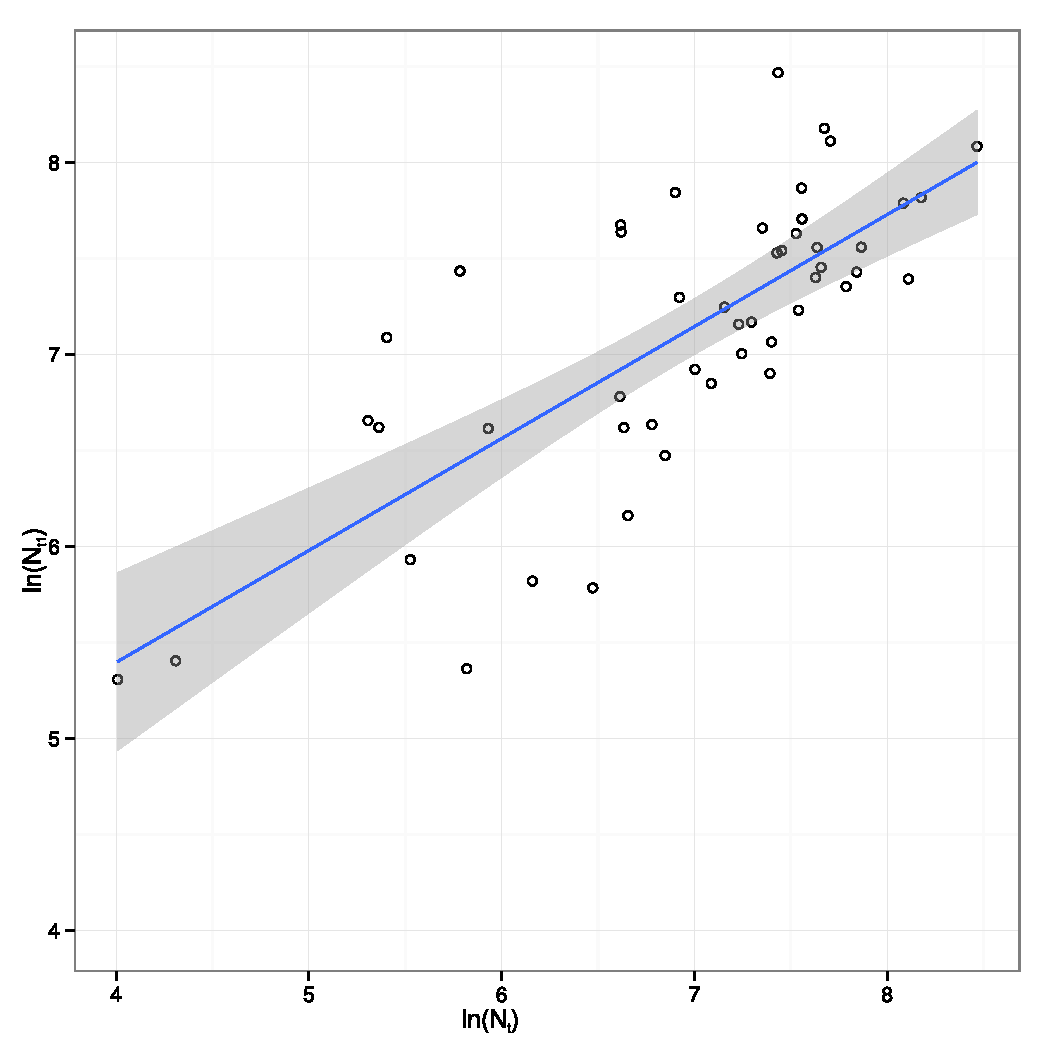
\includegraphics[height=0.4\textheight]{../article_Macoma_dynamic_White_sea/N_vs_temperature/lodNt_vs_logNt1_1.pdf}

		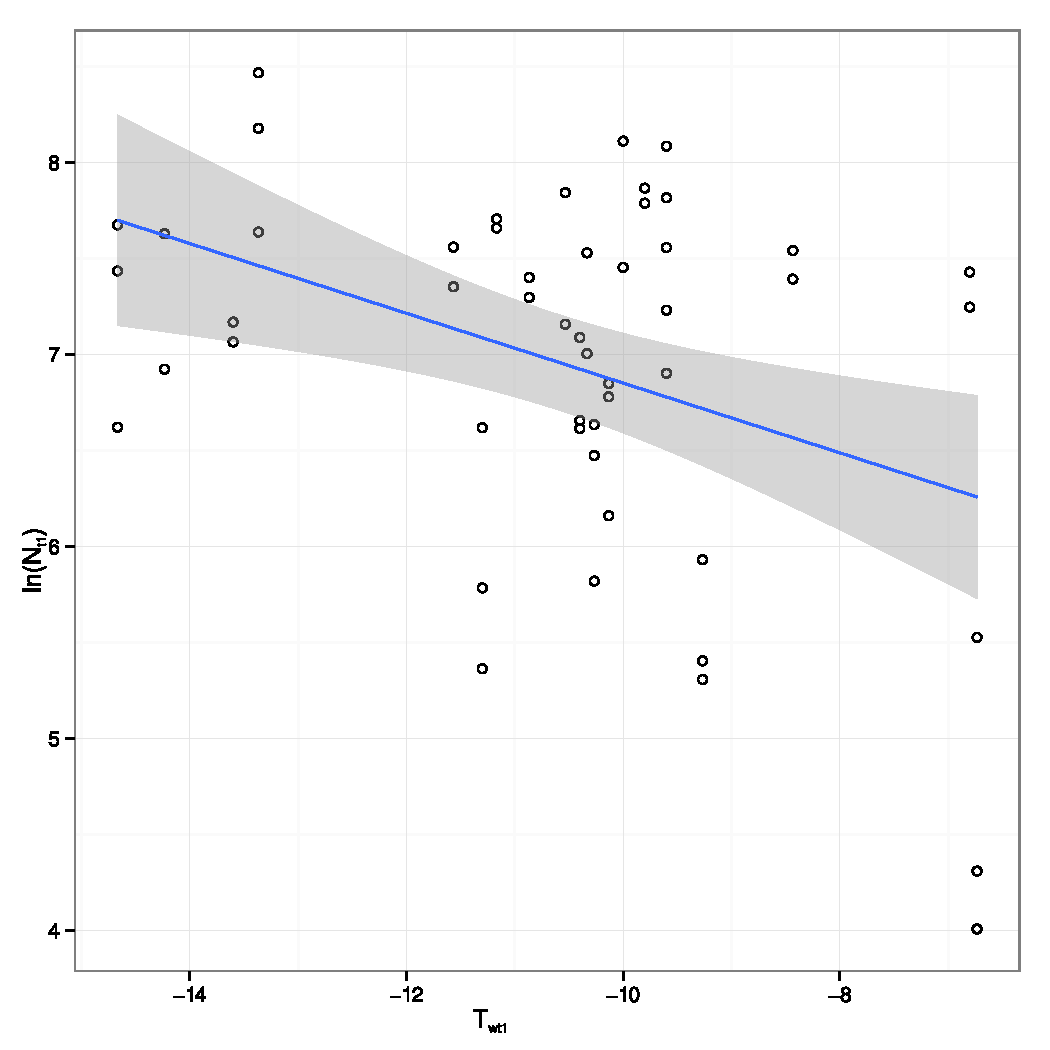
\includegraphics[height=0.4\textheight]{../article_Macoma_dynamic_White_sea/N_vs_temperature/Twt1_vs_logNt1_1.pdf}

	\caption{Зависимость численности  \textit{Macoma balthica} ($\ln(N_{t1})$) от численности в предыдущий год ($\ln(N_{t})$) и зимней температуры ($T_{wt1}$).}
	\label{ris:model_temperature}
	\footnotesize{Показаны линейная модель (синяя линия) и ее 95\% доверительный интервал (серая область).}
	\end{figure}

Полученные данные о влиянии зимней температуры противоречат нашей исходной гипотезе о том, что холодные зимы в Белом море критичны для маком. 
Результаты моделирования позволяют говорить о том, что обилие маком увеличивается после более холодных зим и уменьшается после относительно теплых (рис.~\ref{ris:model_temperature}). 
Данный результат хорошо согласуется с результатами полученными Бьёкема с соавторами (\cite{Beukema_et_al_1998, Beukema_et_al_2009}) для Ваттового моря. 

Для данной акватории было показано, что одним из ключевых факторов, влияющих на пополнение поселений \textit{M.~balthica}, является температура в зимний период. 
Пополнение после суровых зим было больше, чем после мягких. 
Было предложено два механизма, зависимые от зимней температуры: 
1. количество яиц маком, выметанных в апреле больше после холодной зимы, поскольку при низкой температуре меньше уровень обмена, а, значит, меньше потери веса за зиму, и больше энергии остается на продукцию. 
2. Биомасса \textit{Crangon crangon}, одного из важных хищников для маком, была значительно выше после холодных зим. 
При проверке обеих гипотез, было показано, что второй механизм влияет значительно сильнее (\cite{Beukema_et_al_1998, Beukema_Dekker_2014, Dekker_Beukema_2014}). 

В настоящее время у нас нет прямых данных, позволяющих говорить о механизмах влияния температуры на \textit{M.~balthica} в Белом море. 
Проведение аналогий с Ваттовым морем затруднено, поскольку считается, что роль хищников снижается в более полярных сообществах (\cite{Pianka_1966, Freestone_et_al_2011}). 
Возможно, уменьшение обилия маком после теплых зим связано с тем, что при более теплых зимах ледостав менее стабилен, и литораль во время отлива оказывается напрямую подвержена воздействию отрицательных температур воздуха, в то время как в холодные зимы стабильный ледовый покров создает изолирующий слой, и колебания температуры подо льдом оказываются значительно ниже (\cite{Kuznecov_1960}).

\afterpage{\clearpage}


\afterpage{\clearpage}
%%%%%%%%%%%%%%%%%%%%%%%%%
	\subsection{Особенности пополнения поселений \textit{Macoma balthica} в Белом и Баренцевом морях}
Для видов с планктонной личинкой пополнение молодью является основным фактором, влияющим на динамику поселений.
Поэтому мы рассматривали количественные характеристики формирования спата и обилие годовалых особей, как отражения различных стадий процесса пополнения.

%обсуждение
По нашим данным плотность поселения спата была одного порядка на трех исследованных участках ($4-5$~тыс.~экз./м$^2$), но в проливе Подпахта была выше на порядок (более $10$~тыс.~экз./м$^2$). 
Интересно отметить, что высокая плотность спата была отмечена именно в Подпахте, т.е. на участке с минимальной плотностью поселения взрослых особей. 

Учитывая имеющиеся оценки смертности спата нам показалось интересным посмотреть соотношение спата этого года и сеголетков. 
Сеголетками (возраст $1+$) считали особей длиной $1,1-2,0$~мм в соответствии с работой Н.В.Максимовича с соавторами, выполненной в исследованной акватории (\cite{Maximovich_et_al_1992}). 
Смертность спата маком за сезон оценивается в $59.1$\% (\cite{Burkovskiy_et_al_1998}). Полученные расчетные величины представлены в табл.~\ref{tab:spat_rasschet} и \ref{tab:N1_rasschet}.

\begin{table}[p]
\caption{Предположительное пополнение исследованных поселений \textit{Macoma balthica} в $2005$ году, рассчитанные на основе оценки смертности спата.}
\label{tab:spat_rasschet}
\begin{center}
\begin{tabular}{|l|c|c|}
\hline
                & $2005$ (расчет) & $2006$ \\ 
возраст         & $N_{sp}$      & $N_{1+}$  \\ \hline
Сухая салма     & $473$           & $194$  \\ \hline
бухта Лисья     & $415$           & $170$  \\ \hline
пролив Подпахта & $166$           & $68$   \\ \hline
бухта Клющиха   & $351$           & $144$  \\ \hline
\end{tabular}
\end{center}
	\footnotesize{Примечание: $N_{sp}$.~--- плотность поселения спата, экз./м$^2$, $N_{1+}$~--- плотность поселения сеголетков, экз./м$^2$.}

\end{table}


\begin{table}[p]
\caption{Предположительная эффективность пополнения исследованных поселений Macoma balthica к 2007 году, рассчитанные на основе оценки смертности спата.}
\label{tab:N1_rasschet}
\begin{center}
\begin{tabular}{|l|c|c|}
\hline
                & $2006$  & $2007$ (расчет) \\
возраст         & $N_{sp}$      & $N_{1+}$  \\ \hline
Сухая салма     & $4980$  & $2042$          \\ \hline
бухта Лисья     & $4040$  & $1656$          \\ \hline
пролив Подпахта & $4240$  & $1738$          \\ \hline
бухта Клющиха   & $10060$ & $4125$         \\ \hline
\end{tabular}
\end{center}
	\footnotesize{Примечание: $N_{sp}$.~--- плотность поселения спата, экз./м$^2$, $N_{1+}$~--- плотность поселения сеголетков, экз./м$^2$.}
\end{table}

Таким образом, расчетные величины обилия спата в $2005$ году на порядок отличаются от величин, показанных для $2006$ года. 
Возможно, это связано с значительными межгодовыми различиями в пополнении поселений, показанных для других участков (рис.~\ref{ris:dynamic_1year_Kandalaksha}). 
Также это может быть связано с тем, что приведенная оценка сделана для смертности за сезон, и смертность за последующую зиму может значительно занижать нашу оценку пополнения в $2005$ году. 

Размерная структура спата на всех исследованных участках характеризуется мономодальностью. 
Подобные данные были получены М.А. Зубахой с соавторами (2000), однако в данной работе было показано, что мономодальное распределение спата формируется в конце лета. 
Изначально при оседании формируется бимодальная размерная структура, связанная с двумя пиками численности личинок в планктоне, и затем за счет различной скорости роста личинок два пика постепенно сливаются (\cite{Zubakha_et_al_2000}).
На исследованных участках максимальный размер плантиграды имели на участке в бухте Клющиха ($0,4 - 1,5$~мм с модой $0,75$~мм), а минимальный в проливе Подпахта ($0,35 - 0,8$~мм с модой $0,5$~мм). 
Это хорошо согласуется с данными Е. Олафссона, который показал, что на песчаных грунтах нет подавления роста спата взрослыми особями, наблюдаемого на илисто-песчаном грунте (\cite{Olafsson_1989}). 
Участок в бухте Клющиха отличался отсутствием алевритов и пелитов (табл.~\ref{tab:grunt_granulometriya_White}), в то время как остальные характеризовались значительным заилением. 
В $1998$ году на участке Сухая салма к $25$~августа моду формировали особи длиной $0,55 - 0,75$~мм с небольшим преобладанием группы $0,65$~мм (\cite{Zubakha_et_al_2000}). 
По нашим данным к $20$~августа структура поселения была с выраженным пиком при длине спата $0,65$~мкм. 
Разброс размеров в $1998$ году был от $0,35$ до $0,95$~мм, а в $2006$ от $0,3$ до $0,85$~мм, то есть в $2006$ году особи были более мелкие, не смотря на более поздние сроки сбора материала. 

При анализе корреляции количества спата и обилием взрослых особей \textit{M.~balthica} было показано, что с биомассой достоверной корреляции нет, а есть отрицательная с плотностью поселения. 
Между тем, если предполагать трофическую или топическую конкуренцию, то следовало бы ожидать наличия именно отрицательной корреляции с биомассой, поскольку более крупные макомы имеют больший радиус облова и отбирают на себя больший поток энергии (\cite{Olafsson_1989, Zwarts_et_al_1994}). 
Тогда возникло предположение, что такая картина может объясняться взаимодействием спата с более мелкими, но более многочисленными макомами. 
Однако при анализе корреляции плотности поселения спата и количества маком различных размеров это показать не удалось.

Дисперсионный анализ показал, что плотность поселения спата сильно варьирует в зависимости от участка, и фактор участок определяет $45 \pm 6,8$\% вариации. 
Это может быть связано с сильной вариабельностью плотности поселения личинок в планктоне на различных участках (\cite{Maximovich_Shilin_2012}). 
Кроме того, поскольку в данном исследовании не проводилось наблюдение за динамикой оседания спата, то наблюдаемая картина является результирующей оседания и последующего перераспределения маком за счет биссусного дрифта (\cite{Armonies_Hellwig-Armonies_1992, Huxham_Richards_2003}).
Хотя для фактора плотность поселения взрослых маком сила влияния недостоверна, но поскольку анализ силы влияния фактора более слабый, чем дисперсионный анализ, то можно говорить о влиянии плотности поселения взрослых маком на количество спата. Но оценить влияние на имеющемся материале невозможно.

Интересные результаты получились при анализе влияния местообитания и плотности поселения взрослых маком на отдельные размерные группы маком. 
Для особей длиной более $5$~мм характер влияния факторов аналогичен таковому у спата, в то время как для особей длиной $1,1 - 5,0$~мм влияние фактора <<участок>> недостоверно, а влияние плотности поселения взрослых маком больше. 
Можно было бы предположить, что именно количество особей длиной $1,1 - 5,0$~мм определяет плотность поселения маком в поселении, однако корреляция между этими параметрами оказалась недостоверной.

Попытка выявить влияние на плотность поселения спата маком обилия макрозообентоса, что было показано в Ваттовом море (\cite{Flatch_2003}), не показала достоверной связи между данными показателями. 
Возможно, это связано с тем, что в Ваттовом море в исследованных поселениях обилие определялось количеством двустворчатого моллюска \textit{Cerastoderma edule} и пескожила \textit{Arenicola marina}, в то время как в исследованных нами поселениях не было столь крупных и активно изменяющих среду организмов. 

\par\bigskip
В данной работе мы оценивали успешность пополнения беломорских поселений \textit{M.~balthica} по плотности поселения годовалых особей.
Данный показатель варьировал в значительных пределах: от $0$ до $5,5$~тыс.~экз./м$^2$.
Таким образом, исследованные поселения демонстрируют характерную для Белого моря нерегулярность пополнения (\cite{Maximovich_et_al_1991, Maximovich_Gerasimova_2004, Gerasimova_Maximovich_2009}).

Считается, что пополнение локальных поселений массовых бентосных организмов с планктонной личинкой не зависит от количества половозрелых особей в нем, поскольку единый личиночный пул в планктоне формируется за счет всех половозрелых особей в гидрологически-замкнутой акватории (\cite{Maximovich_Shilin_2012}.
Мы попробовали на имеющихся материалах проверить данную гипотезу.
Поскольку для маком в Белом море показано (\cite{Semenova_1980, Maximovich_1985}), что ключевым фактором для возможности половозрелости является именно размер, а не возраст животного, и этот размер для макомы составляет 8 мм, мы оценивали корреляцию плотности поселения годовалых особей с плотностью поселения особей длиной более $8$~мм в предыдущий год (т.е.в год оседания).
Хотя была обнаружена низкая достоверная корреляция данных параметров, очевидно (рис.~\ref{ris:N1year_vs_N8mm}) что разброс данных величин достаточно высокий и влияние данного фактора невелико.
В пользу гипотезы о формировании общего личиночного пула на значительной акватории говорит и синхронность пополнения, наблюдаемая в ряде исследованных поселений (табл.~\ref{tab:Mantel_dynamic_N1y}).
Единственное поселение, для которого не показана синхронность с остальными --- на острове Ломнишном, наиболее удаленном поселении от остальных участков.
Однако прямой связи расстояния со степенью синхронности пополнения поселений обнаружено не было.

В Баренцевом море мы не проводили анализа пополнения, однако по данным размерной структуры можно сделать некоторые выводы.
На Дальнем пляже особи размером $2-3$~мм встречаются ежегодно, хотя бы в единичном количестве.
В данном районе такой размер характерен для маком возрастом $1+$ (\cite{Nazarova_et_al_2010}), таким образом, можно говорить о регулярном пополнении поселений молодью. 
Однако эффективность пополнения различается год от года. 
Наиболее успешные пополнения поселения молодью, по-видимому, происходили в $2005-2007$ годах, что и обусловило увеличение плотности поселения маком в $2006-2008$ годах на данном участке.
Таким образом, значительные межгодовые различия в эффективности пополнения поселений маком молодью характерны как для Белого, так и для Баренцева морей.



\afterpage{\clearpage}
